\documentclass{DeustoFDP}
\usepackage[toc, acronym, nomain]{glossaries}
\usepackage{verbments}
\usepackage{placeins}

\listofpyglistingsname{Algorithm Index}

\hypersetup{
  pdfauthor={Jesús María Sesma Solance},
  pdftitle={Automatic Detection of Repressed Anger from Text Messages},
}

\bibliography{bibliography}
\makeglossaries
\newacronym{ocr}{OCR}{Optical Character Recognition}
\newacronym{svm}{SVM}{Support Vector Machine}
\newacronym{nn}{NN}{Neural Network}
\newacronym{dt}{DT}{Decision Tree}
\newacronym{bnc}{BNC}{British National Corpus}
\newacronym{cnn}{CNN}{Convolutional Neural Networks}
\newacronym{nlp}{NLP}{Natural Language Processing}
\newacronym{sa}{SA}{Sentiment Analysis}
\newacronym{om}{OM}{Opinion Mining}
\newacronym{html}{HTML}{Hypertext Markup Language}
\newacronym{ml}{ML}{Machine Learning}
\newacronym{url}{URL}{Uniform Resource Locator}
\newacronym{occ}{OCC}{Ortony Clore and Collins}
\newacronym{hfw}{HFW}{High Frequency Word}
\newacronym{cw}{CW}{Content Word}
\newacronym{knn}{KNN}{K-Nearest Neighbors}
\newacronym{apa}{APA}{American Psychological Association}

\begin{document}

\frontmatter
\pagestyle{plain}

\begin{titlepage}
  \newgeometry{left=0cm,right=0cm,bottom=0cm,top=0cm}\thispagestyle{empty}
  
\includegraphics{figures/frontpage-comp}
  \restoregeometry
\end{titlepage}
\cleardoublepage

The growth in the usage of social media, microblog and review platforms has resulted in a significant increase of the access to short text messages that reflect individual's opinion and feelings. Automatic detection of people's emotions has a wide range of applications such as producing systems that measure the satisfaction of customers and thus help companies to improve their products or services. This research project focuses on detecting anger, an emotion that is relative difficult to detect compared to other sentiments due to the usage of linguistics figurative language techniques, such as irony, that intends to communicate the opposite of what it is literally said.
To this purpose, a review of the state of the art has been made and an experiment using not only traditional machine learning techniques, such as Neural Networks, K-Nearest Neighbor and Support Vector Machines, but also Deep learning algorithms has been conducted in an open social network like Twitter.
The proposed methods define the repressed anger detection as a classification problem and to solve it, the task is divided into two subtasks that complement each other. The first focuses on explicit anger detection, while the second subtask's goal is to detect irony. The system make use of selected featured based on characteristics properties of English language and studies emotion and irony in psychology. The model is composed on features such as: frequency of words, style in written and spoken languages, intensity of adverbs and adjectives, structure of the document, use of emoticons, synonymy, ambiguity and the contrast of sentiment and negative situation.

Keywords
Anger Detection, Machine Learning, add 3 more descriptors.

\cleardoublepage\tableofcontents
\cleardoublepage\listoffigures
\cleardoublepage\listoftables
\cleardoublepage\listofpyglistings

\mainmatter
\pagestyle{phdthesis}

\chapter{Introduction}

\begin{itemize}
  \item Introduction
  \begin{itemize}
    \item Get the important points of the state of art referring to sentiment analysis, repressed anger detection.
    \item Explain the hypothesis to be worked out in the thesis.
  \end{itemize}

  \item Planning and Methodology [OK]
  \begin{itemize}
    \item Explain the plan. [OK]
    \item Explain the methodology. [OK]
    \item Show the schedule. [OK]
  \end{itemize}

  \item State of art
  \begin{itemize}
    \item Explain that sentiment analysis is.
    \item Explain what emotion analysis is, compared to previous point.
    \item Explain previous work.
    \begin{itemize}
      \item Previous work in anger detection.
      \item Previous work in irony detection.
    \end{itemize}
    \item Explain the that the project will focus on resolve the issue as a text classification problem.
    \begin{itemize}
      \item Classification Techniques 
      \item Fundamentals of Classification 
      \item General classification problem solving
      \item Explain the algorithms I used to make tests in WEKA.
      \item Explain Deep Learning.
      \begin{itemize}
        \item Explain Convolutional neural networks.
      \end{itemize}
    \end{itemize}
  \end{itemize} 

  \item Development
  \begin{itemize}
    \item Early development on the exploration phase.
    \begin{itemize}
      \item WEKA text classification testing.
    \end{itemize}
    \item Explain that on SemEval they said that the best scoring system were using DL and is becoming trending. General Problem Solving techniques (NPL) in Deep Leaning perform better that those that focus on resolving in depth focusing on the topic.
    \begin{itemize}
      \item Change to Deep Learning Development.
      \item Explain the usage of architecture that Yoon Kim uses. (Previously explained in SoA)
      \item Explain the process to detect repressed anger. (The system I made starting from dataset merging, ending with merge of 2 classification output.) Simple diagram.
      \begin{itemize}
        \item Dataset searching and generation.

          --> Developed a tweet downloader for IDs.

        \item Word2vec (needed for CNN)

          --> Model used for Word2vec.
          
          --> Spell checking
          
          --> Slang dictionaries (difficulty on when to process the word. Detect Slang)
          
          --> Usage of Stopwords.

        \item CNN classifiers

          --> hyperparams used.

        \item Classification output merge.
        
        --> Due to the labels in the dataset cannot use ensemble learning and use a 2x2 matrix to match everything.
        
        --> Develop a automatic Google forms and how to process them back to the original dataset.
      \end{itemize}
    \end{itemize}
  \end{itemize}

  \item Research Framework
  \begin{itemize}
    \item Searching datasets, or create one, automatically.
    \item Manual labeling used to final prediction process.
  \end{itemize}

  \item Results
  \begin{itemize}
    \item Google Model
    \begin{itemize}
      \item Explain the final result plus each classification independently.
    \end{itemize}
    \item Twitter Model
    \begin{itemize}
      \item Explain the final result plus each classification independently. 
    \end{itemize}
    \item Spell checking
  \end{itemize}

  \item Conclusion and Future Work
    \begin{itemize}
      \item Different approach now that manual label data is obtained.  (Semi-supervised learning) 
    \end{itemize}
  
  \item Self-assessment
  \begin{itemize}
    \item writing.
  \end{itemize}
\end{itemize}
\chapter{Planning and Methodology}

In order to accomplish the Master's thesis during the established period of eight months, the following plan will be followed:
\begin{enumerate}[label=\textbf{\arabic*}.]
    \item \textbf{Exploratory phase:} this period of time will consist in searching and studying the literature related to the research field in order to build a solid theoretical framework on which support the rest of the investigation. Even though this process is presented as a isolated task, it is an fundamental activity that will be executed continuously throughout the whole project.
    \item \textbf{First contact with the technology:} after having reviewed the first phase of the state of art and checked the advantages or limitations of each architecture, the first empirical tests will be done. These experiments will serve to for a better understanding of the literature read in the exploratory phase and to observe how they behave with the gathered sample data.
    \item \textbf{Specification and design of the solution:} in this phase, based on the knowledge gathered from the empirical tests in the last point and the relevant literature that has been constantly read, the requirements of the solution that best results can achieve for this research topic will be specified.
    \item \textbf{Design of the functional prototype and evaluation:} after the requirements gathering, during this task, a prototype that justify all the steps followed this far will be developed, and evaluate its performance.
    \item \textbf{Thesis document writing:} Finally all the relevant knowledge that has been required to complete this research will be gathered, the procedure to develop the system will be described and the conclusion and future work on this topic will be written down altogether, resulting in this master's thesis document, that will be refined until its laster submission and defense.
\end{enumerate}

The figure \ref{fig:methodology} illustrates the methodology used during the investigation process, in which the results obtained from the prototypes might not be satisfactory or could lead to formulate new questions. To solve those doubts a redesign of the system may be needed. In addition, after reporting the results to project supervisor, new relevant information might be provided. This information has to be added to the knowledge obtained from previous state of the art review and reanalyze if the proposed solution requirements are still valid. 

\begin{figure}[!htp]
  \center
  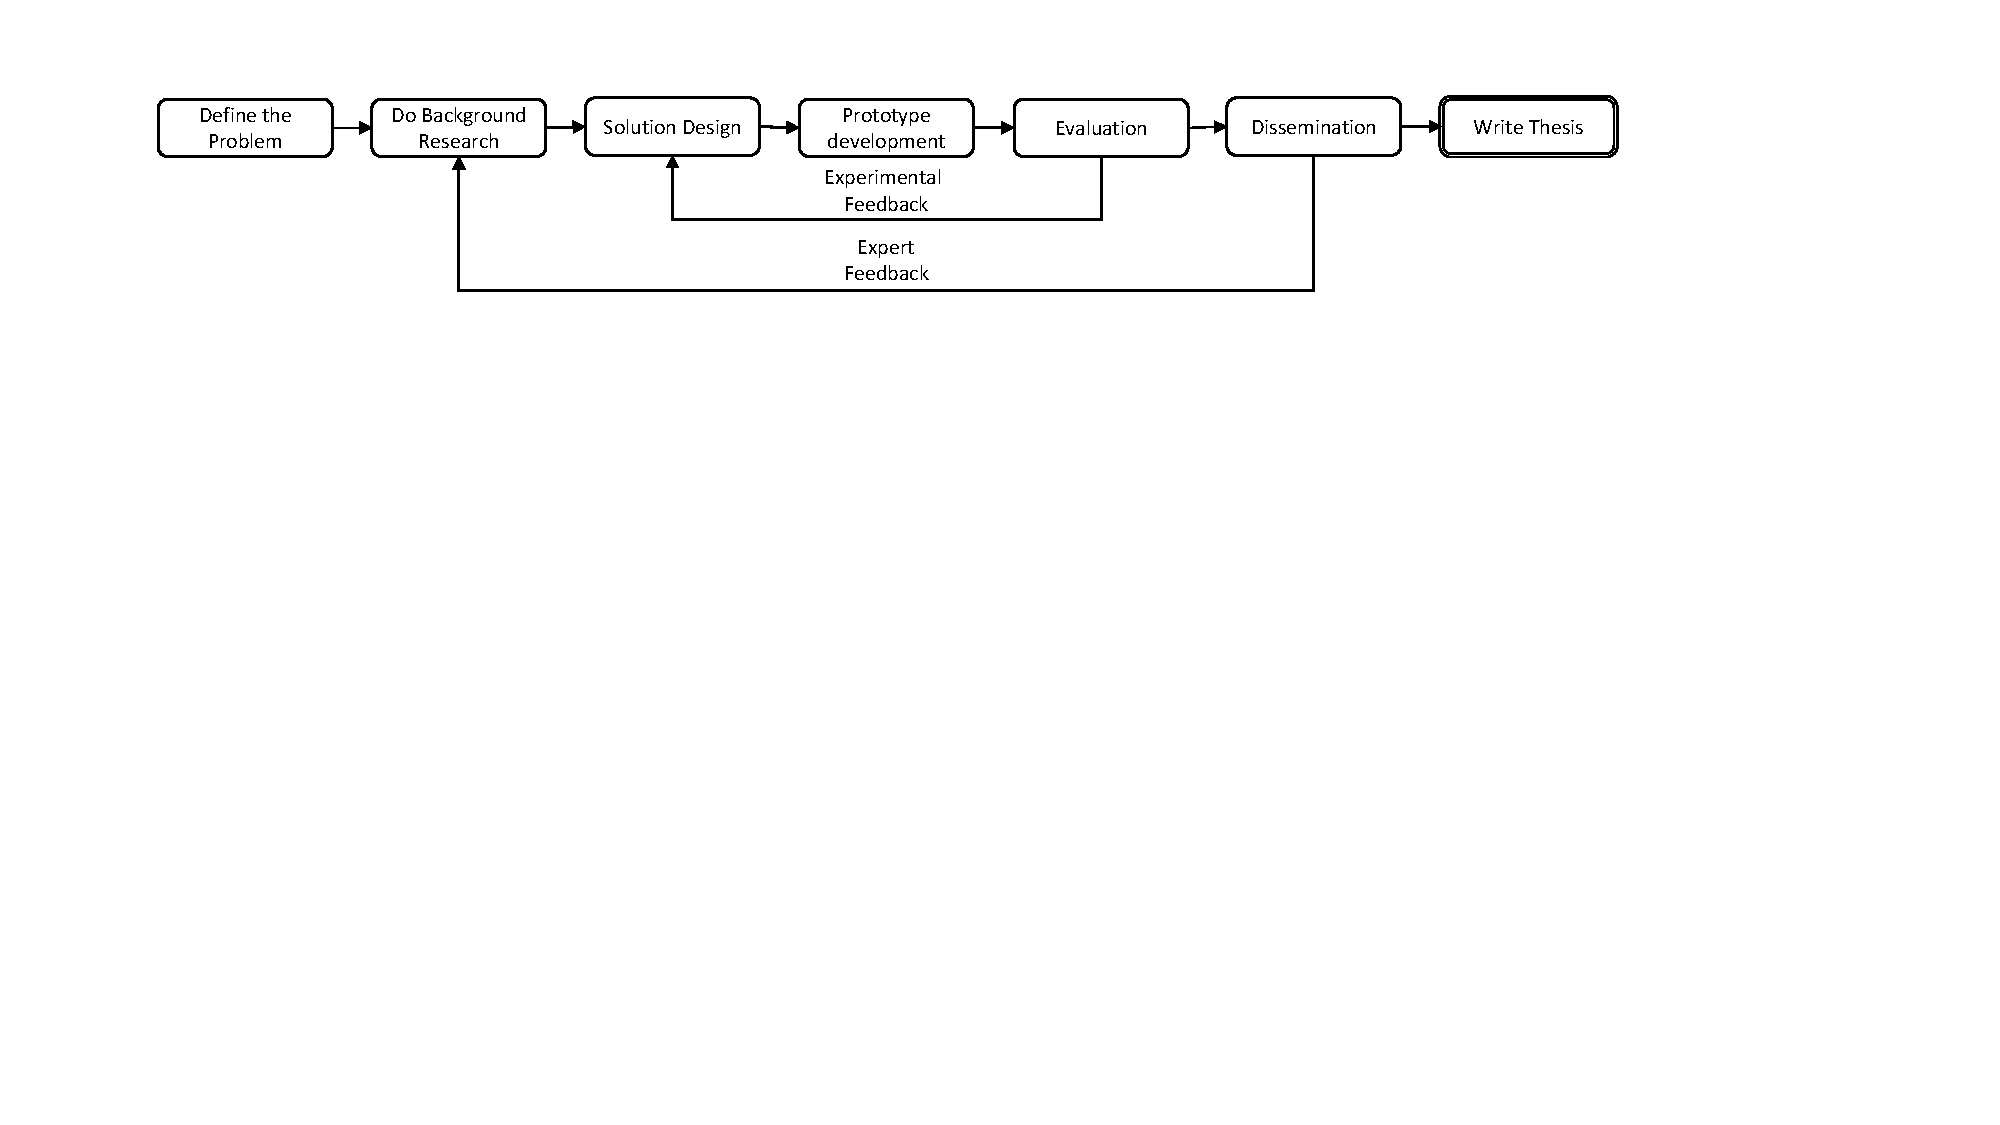
\includegraphics[width=1\textwidth]{figures/scientific_methodology}
  \caption{Methodology}
  \label{fig:methodology}
\end{figure}
\chapter{State of art}

The aim of this chapter is to conduct a study of the state of the art of automatic detection of repressed anger by first analyzing the current state of sentiment analysis and emotion detection, which are the fundamentals to detect anger and irony and thus, repressed anger.

% !TeX root = repressed-anger.tex

\section{Sentiment Analysis}
\label{sec:sentiment_analysis}

\acrfull{sa}, sometimes referred as \acrfull{om}, is the field of study that aims determine the attitude of the author respect to some topic. During the last decade, due mainly to the rapid increase of the social media, the research of this area, which includes linguistics and \acrfull{nlp}, has gain more relevance as it has a wide range of applications that can be used commercially.

Almost the human actions are influenced by opinions. A practical example of this behavior that get repeated in daily basics occurs when before making a decision we want to know other' to contrast our thoughts. In business, when an organization requires to public or consumer opinion, it conducted different types of surveys to gather this information. However, nowadays we do not precise to ask personally to people around us to discuss about a product. Thanks to micro-blogs, Twitter and reviews in social networks, we can broaden the amount of external opinions for decision making. Due to the amusing amount of information available, sometimes we could face some challenges, such as finding reliable sources summarizing and filtering the relevant information. The same way we consume this information, companies also search for new ways to obtain and process such information efficiently without human intervention, to achieve this automated analysis is needed\cite{liu2012sentiment}.

\subsection{Tasks}
\label{subsec:sentiment_analysis_tasks}

\begin{figure}[!htp]
  \center
  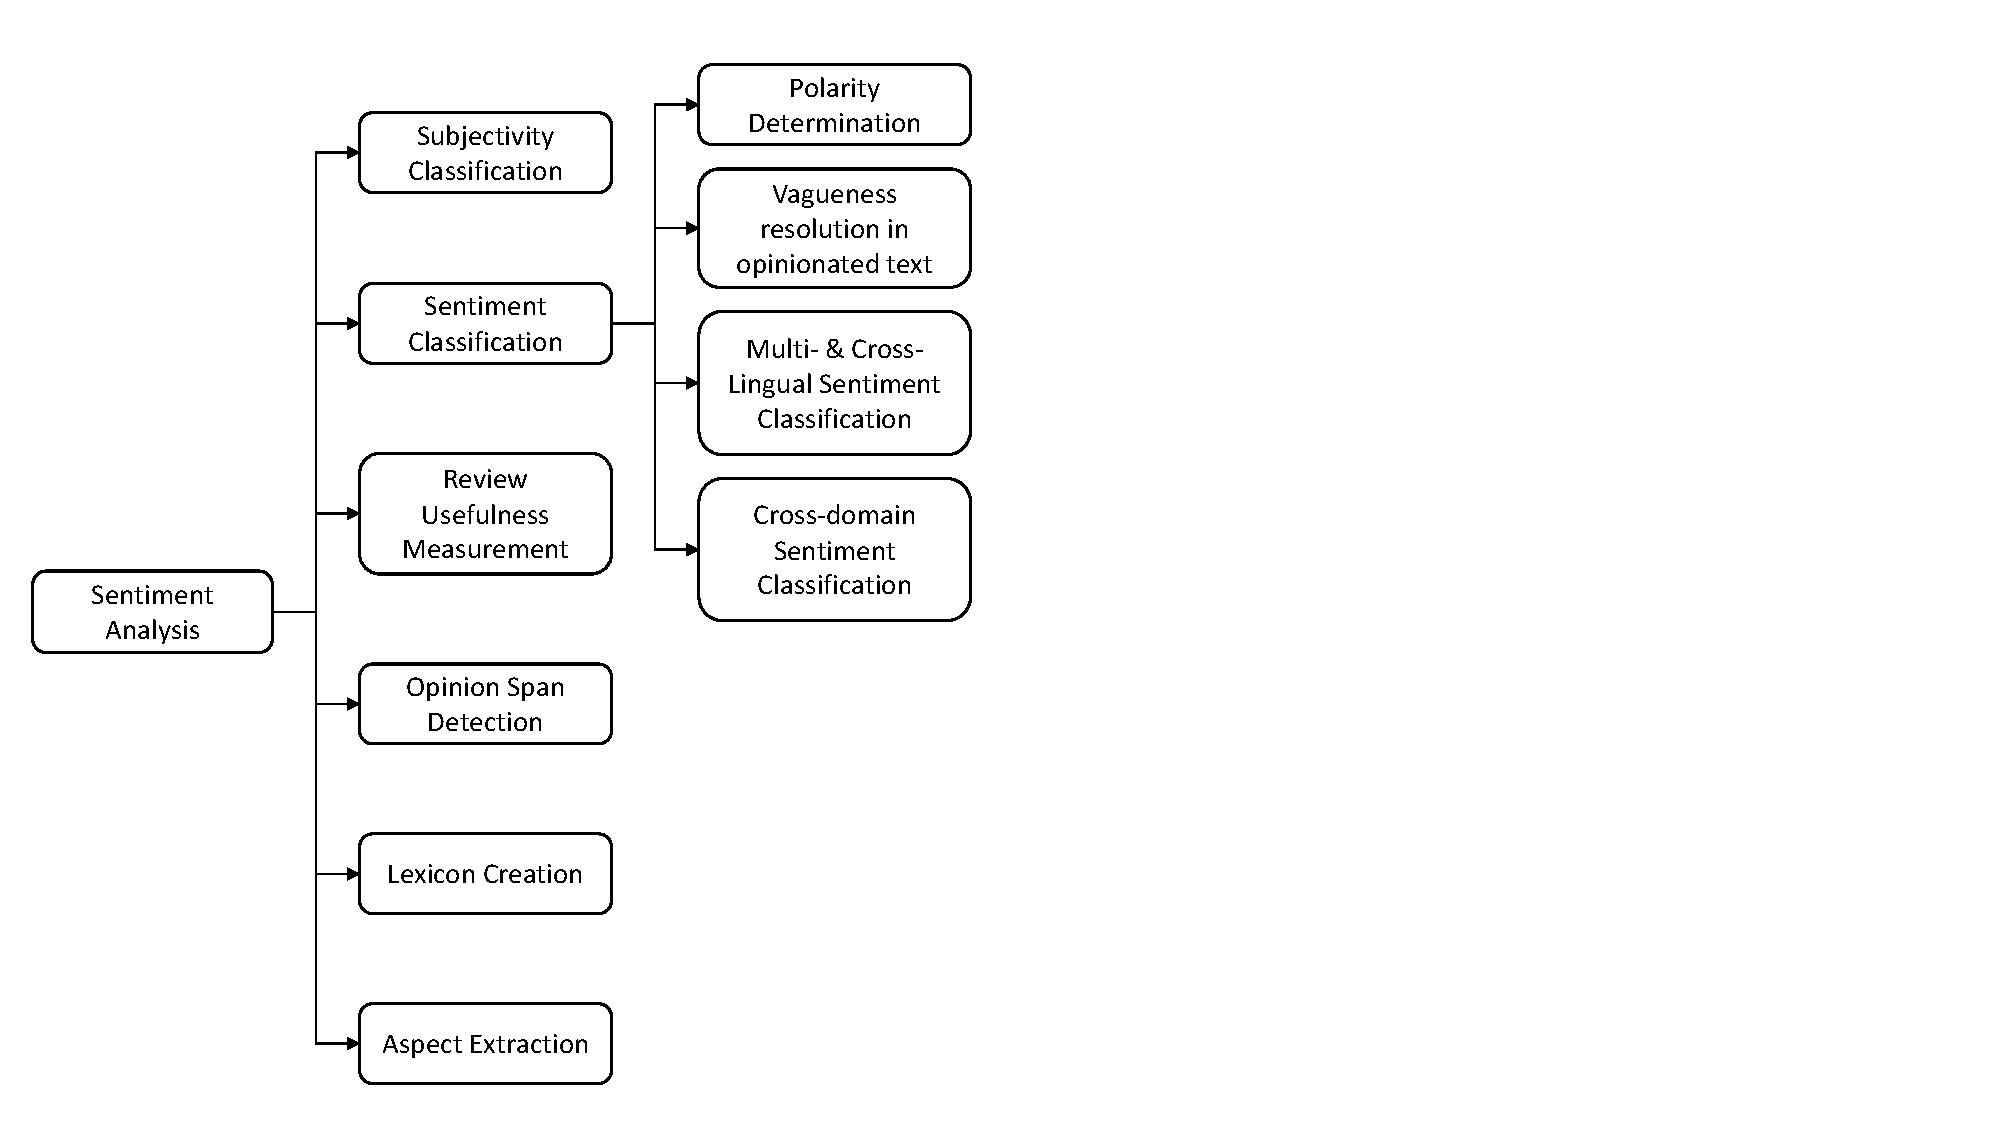
\includegraphics[width=1\textwidth]{figures/sentiment_analysis_tasks}
  \caption{Sentiment analysis tasks.}
  \label{fig:sentiment_analysis_tasks}
\end{figure}

Depending on the problem definition, different tasks have been defined related to sentiment analysis. According to \cite{ravi2015survey}, after the revision of more than three hundred papers related to this topic, the survey carried out concludes that the main tasks can be categorized as (a) subjectivity classification, (b) sentiment classification, (c) review usefulness measurement, (d) opinion spam detection, (e) lexicon creation and (f) aspect extraction, as shown in the figure \ref{fig:sentiment_analysis_tasks}. 

\subsubsection{Subjectivity classification}
\label{subsubsection:subject_classification}

According to \cite{montoyo2012subjectivity}, subjectivity classification aims to determine the "private state" of the author of a text. The Subjectivity analysis is the process of distinguish objective language from the opinion oriented. Even though there is much less literature about this field compared to other \acrshort{sa} task, it has proven to be more difficult than determine the measuring the polarity of a document and, thus, improvements achieved in this field will positively impact on sentiment classification.

\subsubsection{Sentiment classification}
\label{subsubsection:sentiment_classification}

Sentiment classification consist in determine the orientation of a sentiment of a given text into two or more classes. This classification has been performed in multiple classes, such as, binary (positive or negative), ternary (positive, neutral and negative), n-ary, \cite{nakov2016semeval}, among others.

\subsubsection{Review usefulness measurement}
\label{subsubsection:review_usefulness_measurement}

TODO

\subsubsection{Opinion spam detection}
\label{subsubsection:opinion_spam_detection}

TODO

\subsubsection{Lexicon creation}
\label{subsubsection:lexicon_creation}

TODO

\subsubsection{Aspect extraction}
\label{subsubsection:aspect_extraction}

TODO

To solve all these problems in the most efficient way, multiple approaches have been conducted, such as \cite{tripathy2016classification} ; \cite{mullen2004sentiment} or \cite{pouransari2014deep}. The figure \ref{fig:sentiment_analysis_approaches} illustrates which techniques have been used for each previously named categories.

\begin{figure}[!htp]
  \center
  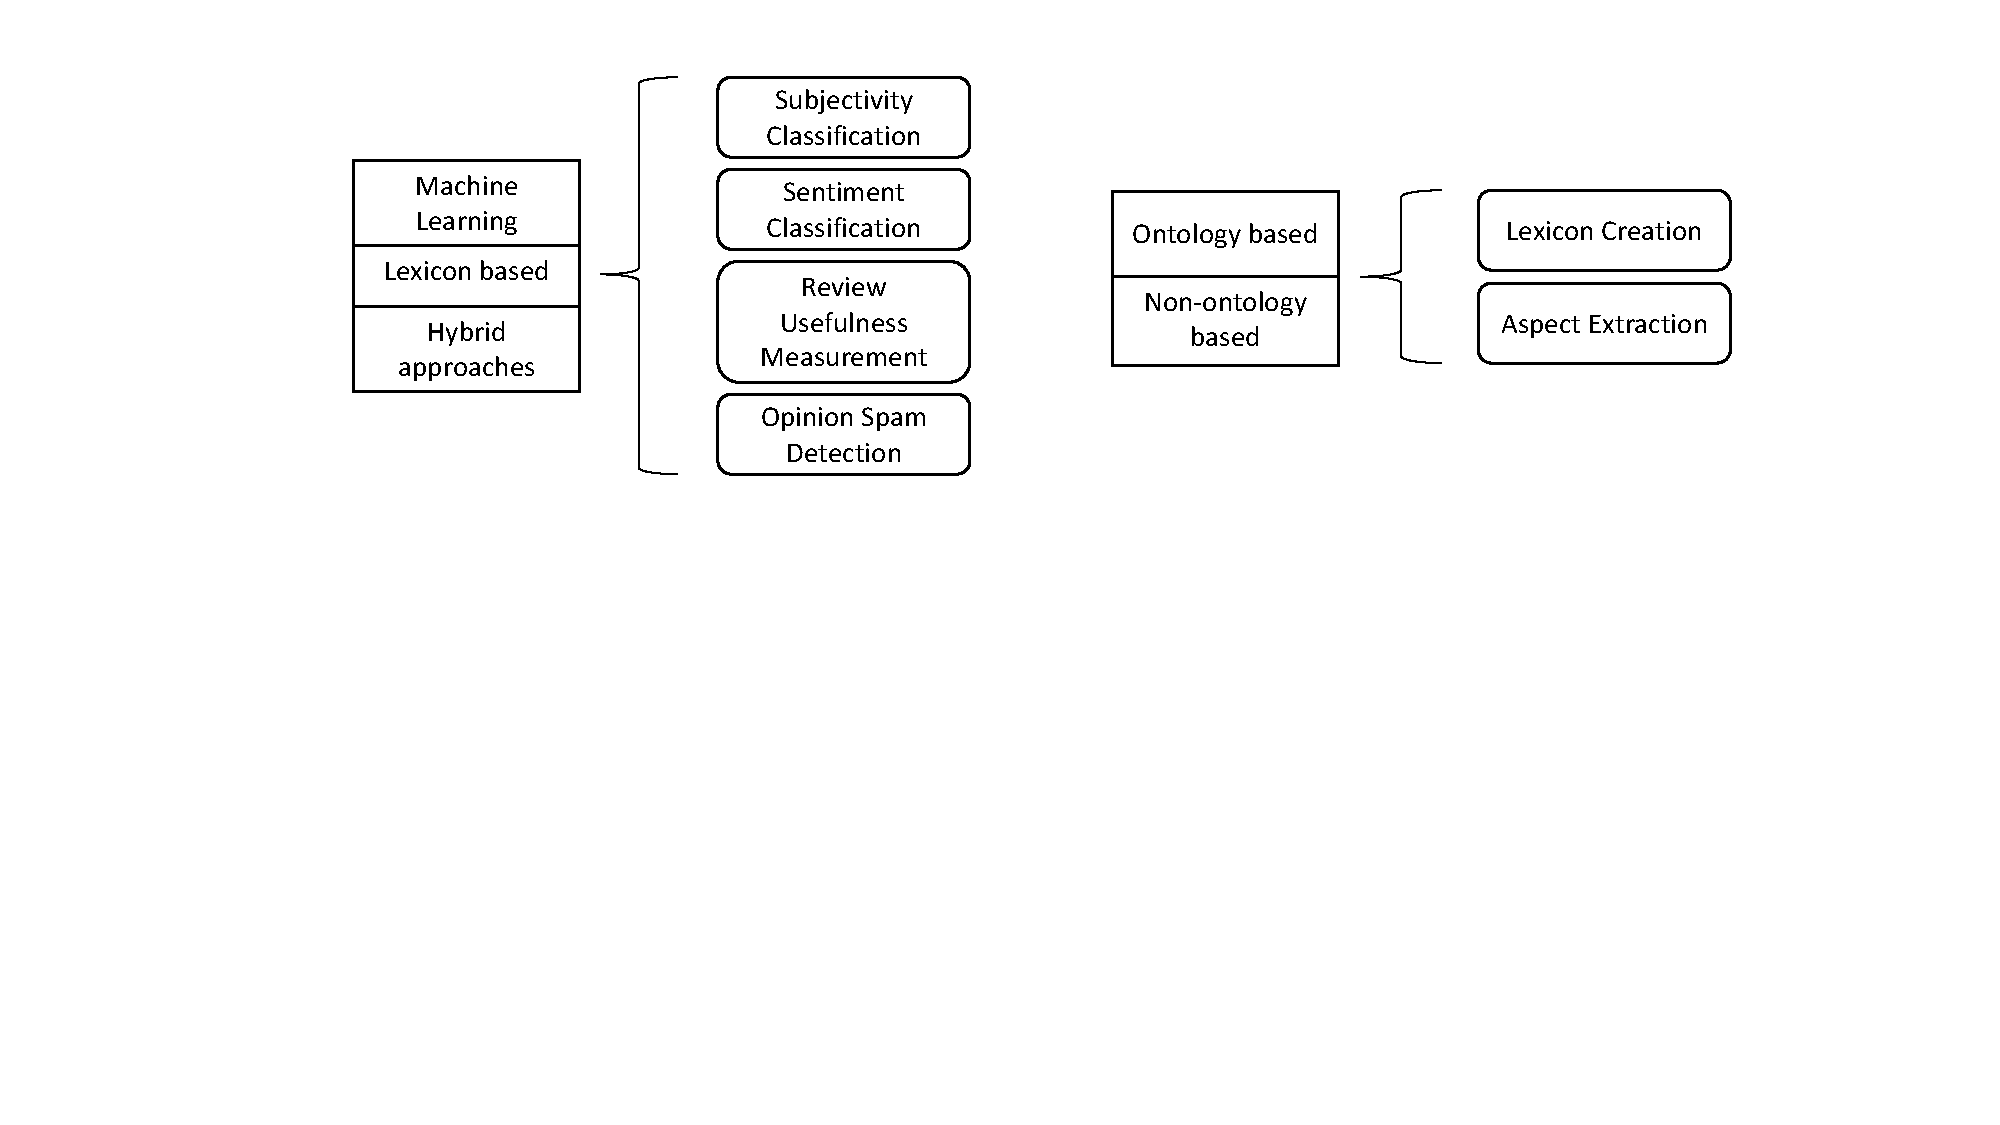
\includegraphics[width=0.9\textwidth]{figures/sentiment_analysis_approaches}
  \caption{Sentiment analysis approaches for each task.}
  \label{fig:sentiment_analysis_approaches}
\end{figure}

\FloatBarrier

\subsection{Techniques}
\label{subsec:sentiment_analysis_techniques}

TODO\cite{thakkar2015approaches}

\begin{figure}[!htp]
  \center
  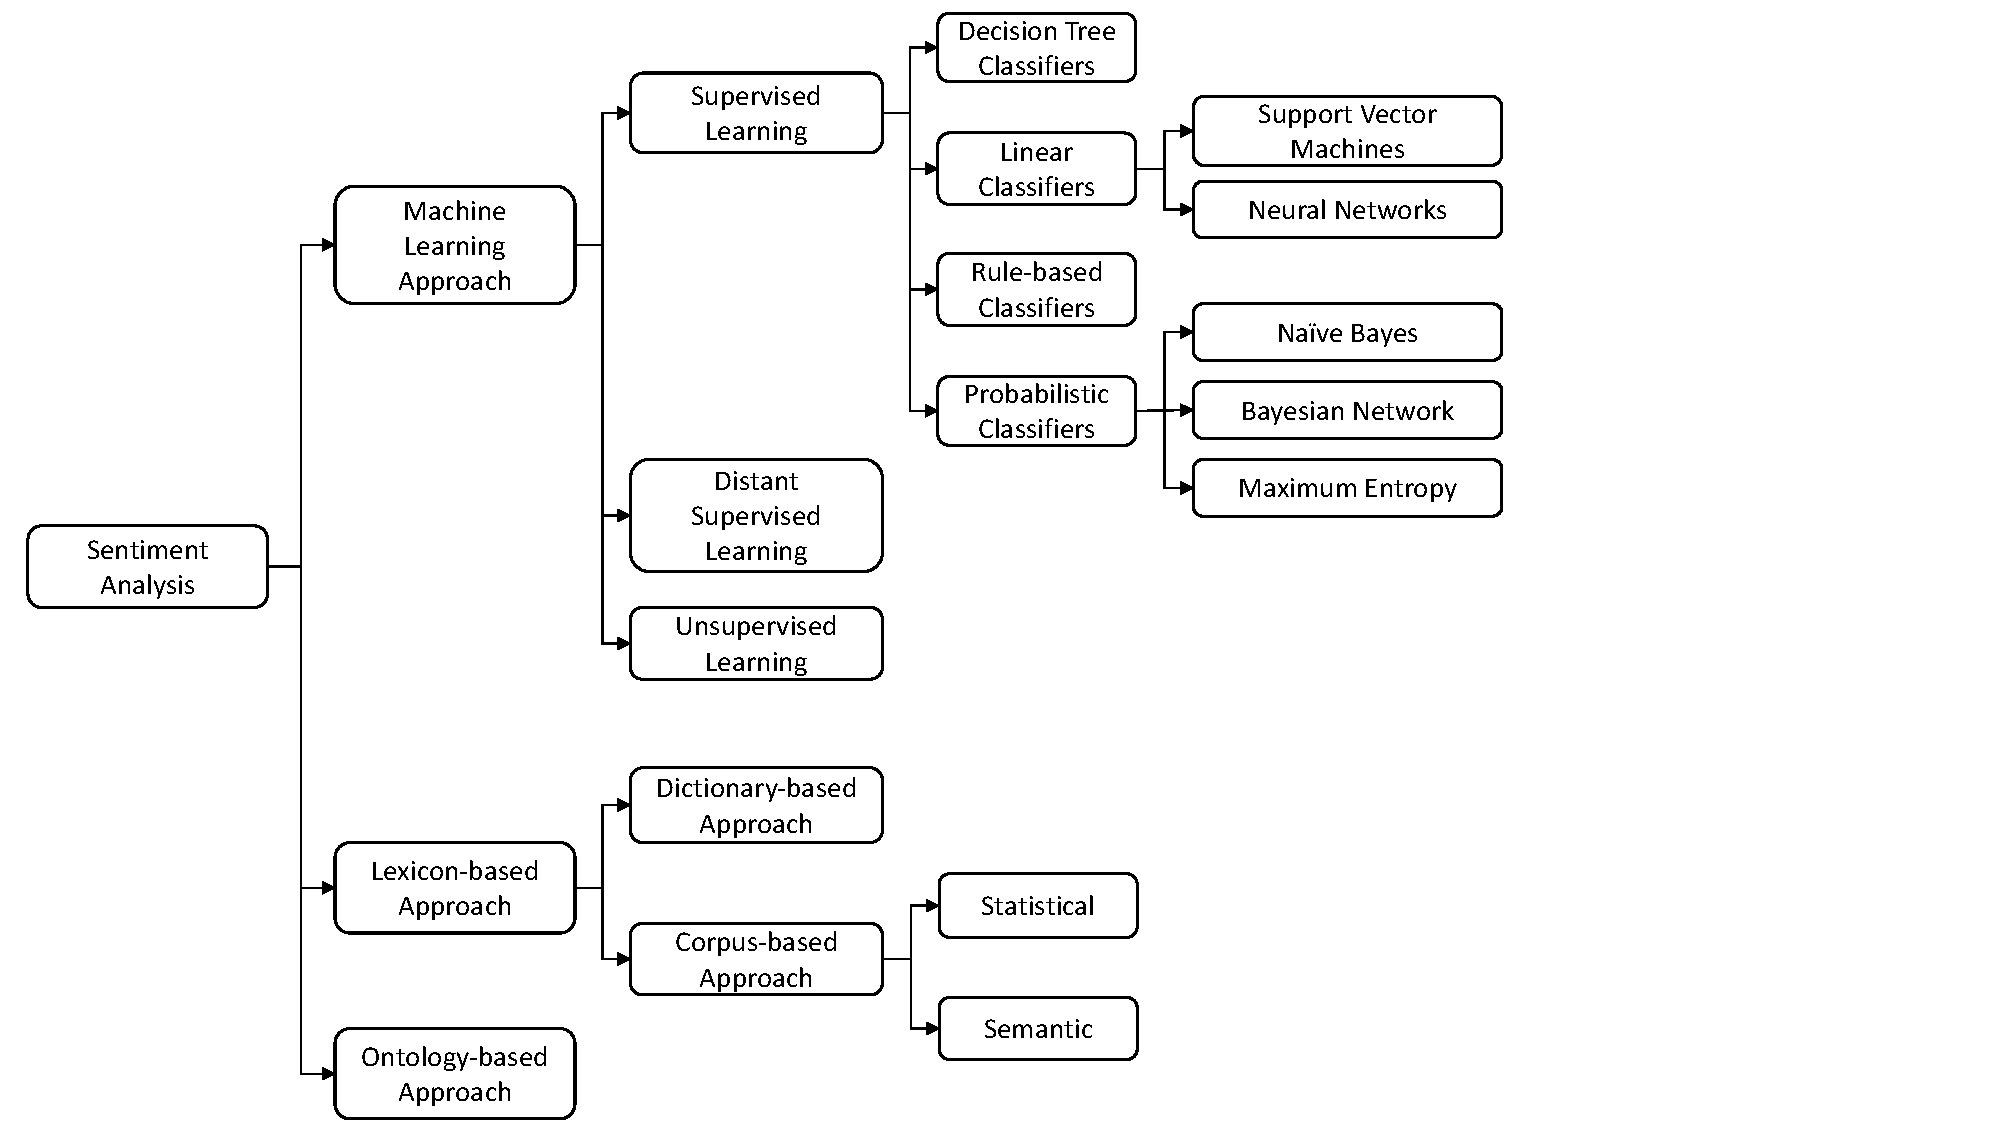
\includegraphics[width=1\textwidth]{figures/sentiment_analysis_techniques}
  \caption{Sentiment analysis techniques\cite{medhat2014sentiment}.}
  \label{fig:sentiment_analysis_techniques}
\end{figure}
% !TeX root = repressed-anger.tex

\section{Emotion Detection}
\label{sec:emotion_detection}

Emotion detection has been always a important field of study in neuroscience and psychology. Several experiments have been conducted to recognize emotions from face expressions, voice and body gestures, such in \cite{bassili1979emotion}; \cite{banziger2009emotion} and \cite{gunes2007bi}. However, these features are not always available and thus, the detection of emotion from text has gain relevance during the last decade.

Emotion detection from text documents is closely related to \acrshort{sa}. As explained in \ref{subsubsection:sentiment_classification}, sentiment classification task consists on determine the polarity of a given text into two or more classes. Emotion detection also fits this description, since this field of study is conducted by classifying a given document into predefined emotion labels. The definition of these labels are based on previously presented emotion models, which consist on application psychological and neuroscientific theories to represent emotions. One of the first model defined was proposed by Paul Ekman, on 1972, composed by six basic emotions, \textit{``happiness, sadness, fear, anger, surprise and disgust''}, and has been used in multiple face recognition systems that has become the base for emotion detection from text \cite{StevenEmotion2011Classification} as its definition has resulted to be the most semantically diverse \cite{bann2013conceptualisation}.

\begin{figure}[!htp]
  \center
  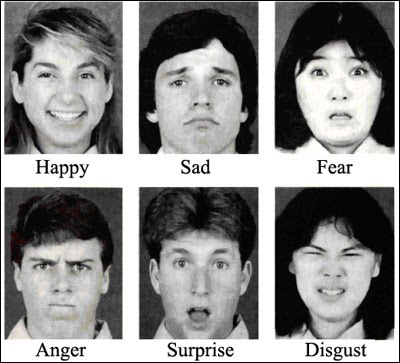
\includegraphics[width=0.67\textwidth]{figures/emotions_ekman}
  \caption{Ekamn's basic emotions, image extracted from Expressions, Emotions and Emblems, Google Sites.}
  \label{fig:ekman_basic_emotions}
\end{figure}

Since then, more interpretations have been made regarding the representation of the emotions as shown in \cite{cambria2012hourglass}. Ekman himself added his list 11 new emotions stating that not all of them could be represented by facial expressions. In 1980, Robert Plutchik created another bi-dimensional model (see figure \ref{fig:plutchik-wheeel}) known as wheel of emotions that defined eight basic bipolar emotions with different levels of intensification and could be combined among them. \acrfull{occ} designed in 1988 a model in which emotions were driven by an agent, based on the premise that \textit{``emotions are not themselves linguistic things, but the most readily available non phenomenal access we have to them is through language''} \cite{binali2010computational}. The model included 22 emotion categories that aimed to \textit{``model humans in general''} \cite{binali2010computational}. \acrshort{occ} enables the study of emotions as classes that share the same feeling, instead of specific words, proving that this \textit{``is a theory of emotions and not a theory of the language of emotions''} \cite{binali2010computational}. For more information, authors of \cite{binali2012emotion} analyze the state of art of the emotion models and the techniques used to generate them.

\begin{figure}[!htp]
  \center
  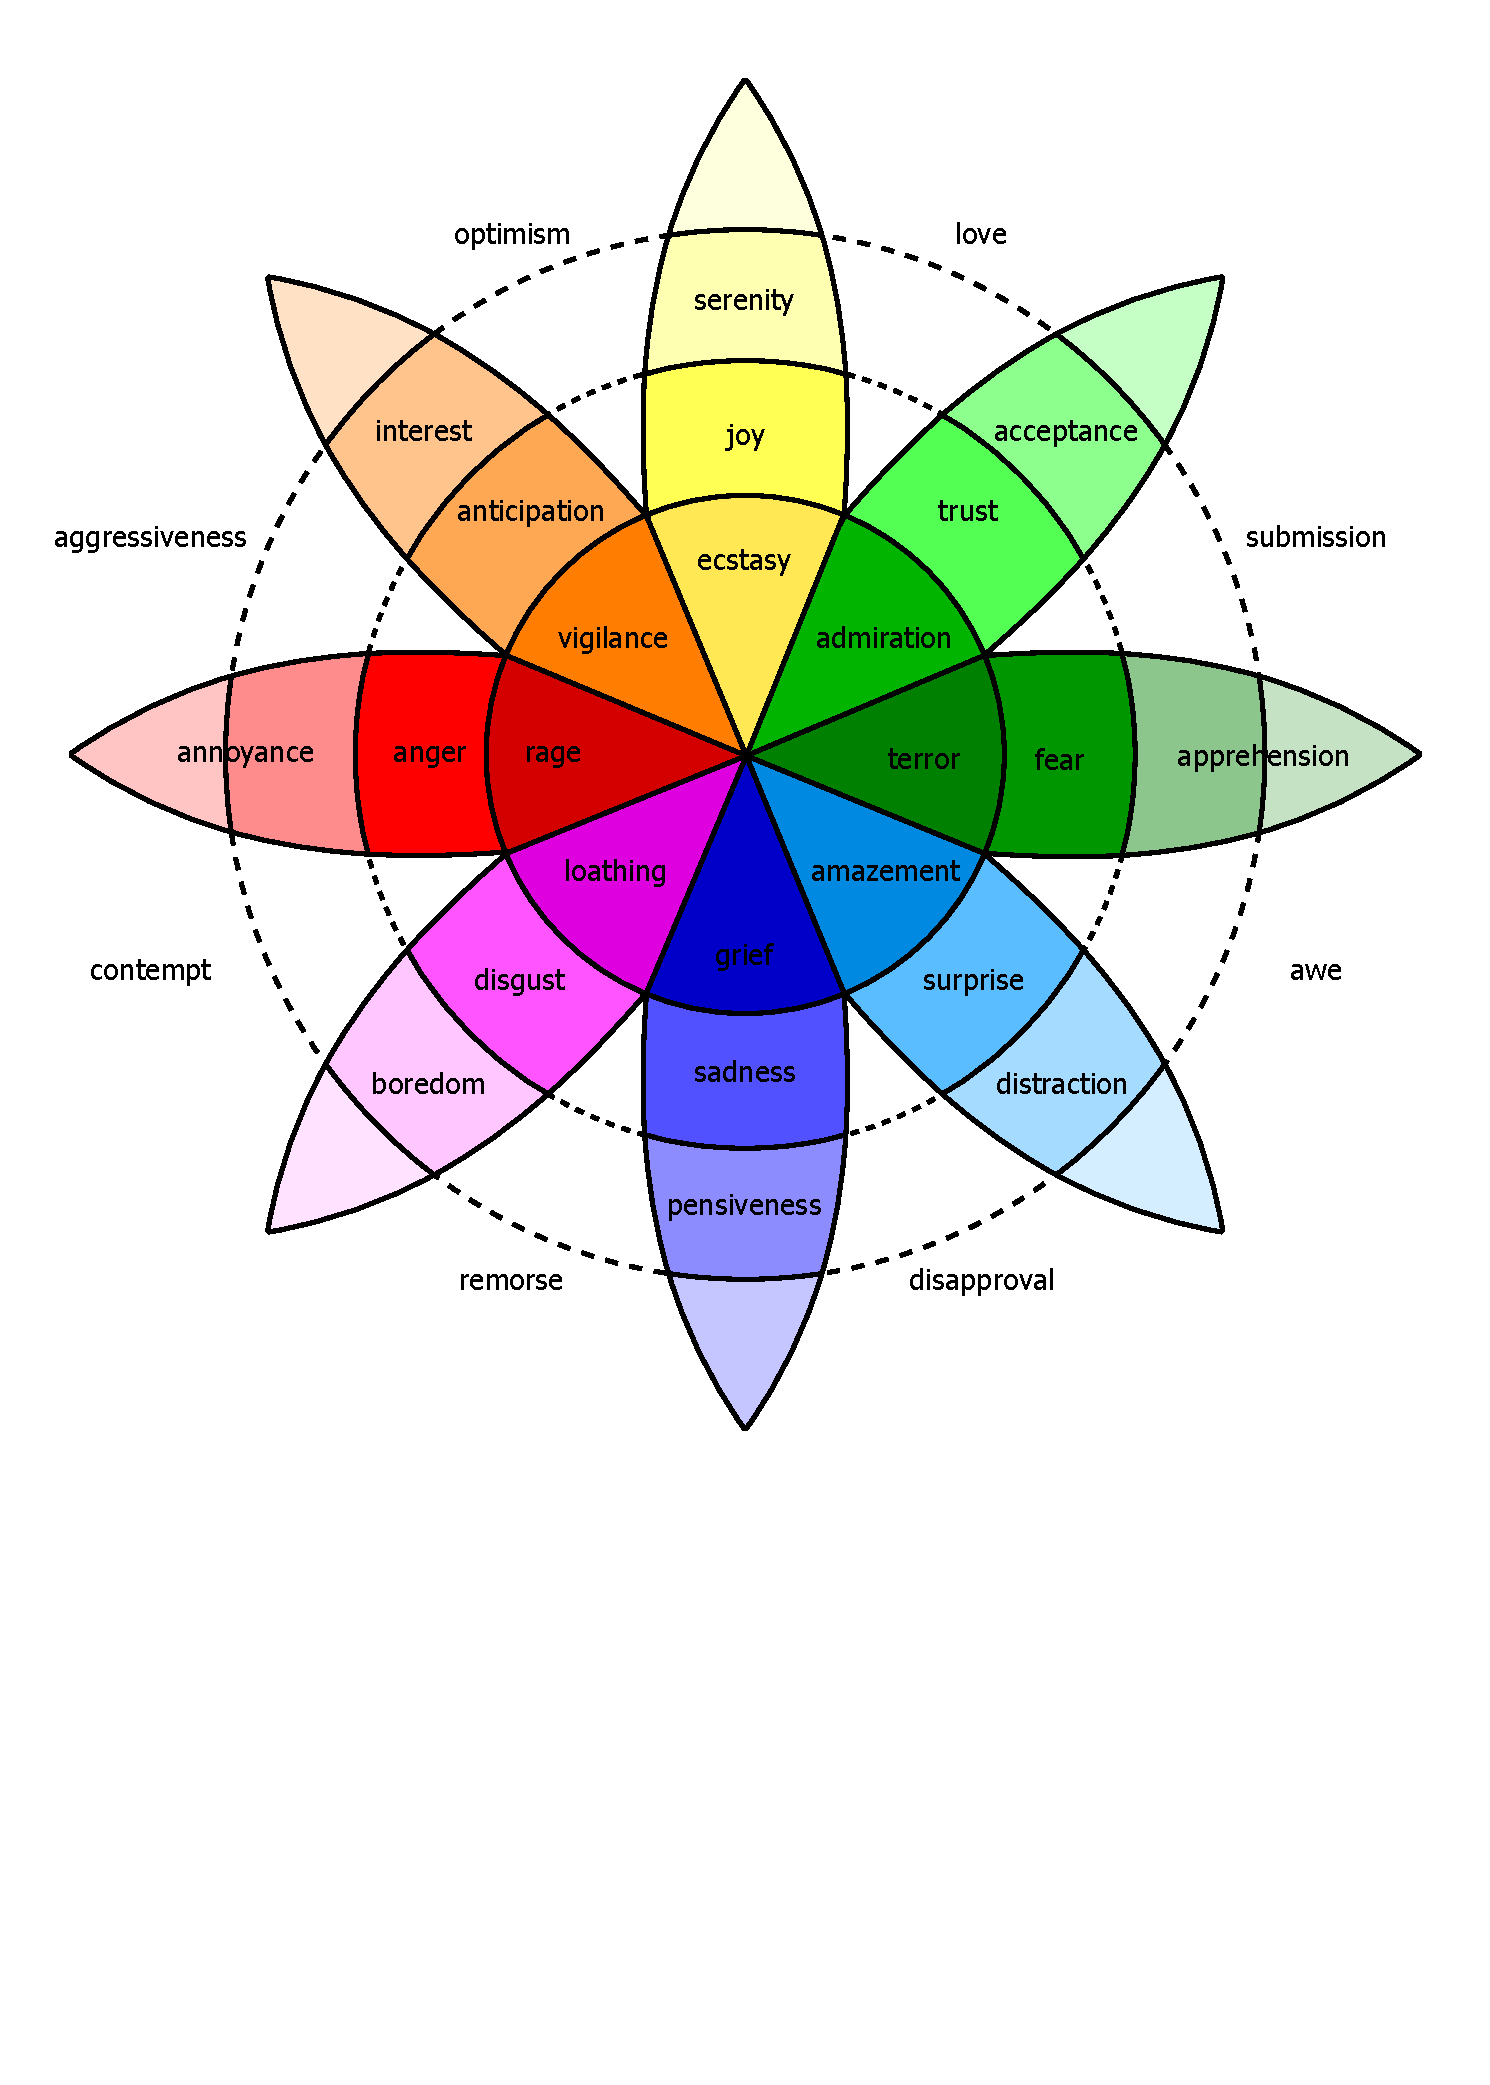
\includegraphics[width=0.67\textwidth]{figures/plutchik-wheel}
  \caption{Plutchik's emotion wheel, image extracted from Wikipedia's public domain.}
  \label{fig:plutchik-wheeel}
\end{figure}

Emotion classification tasks shares the same principles as \acrshort{sa}, and thus, the techniques used are mainly \acrshort{ml}, lexicon-based and hybrid approaches previously explained in section \ref{subsec:sentiment_analysis_techniques}.
% !TeX root = repressed-anger.tex

\section{Previous Work}
\label{sec:previous_work}

The study of anger and its management has been studied since ancient times. According to \acrfull{apa}, anger is \textit{``an emotion characterized by antagonism toward someone or something you feel has deliberately done you wrong''} \cite{angerAPA}. Anger is a normal emotion all human experience. Modern psychologists have studied the health effects that may derivate from anger suppression, such as shown in \cite{kemp1995anger} and \cite{hall1899study}, linking it to a more extremist and sarcastic personality. This research aims to find the answer to the question: \textit{``Can the repressed anger be detected in text?''}. Based on the definition of personality of a subject that has experienced repressed anger, the problem formulation has been simplified into finding negative messages influenced by the anger that is covered by a layer of sarcasm. The following subsections present a brief summary of the research conducted in the detection of anger and sarcasm.

\subsection{Anger}
\label{subsec:anger}

As explained in section \ref{sec:emotion_detection}, the increase of the usage of social media and computational viability to process all the publicly available data has enable the detection of emotions from text. However, as there is not literature that focuses on anger emotion, this section will briefly enunciate the approaches researched to classify emotions that contain anger as target label.

In 2007 during international workshop of evaluations of computational semantics analysis system, known as SemEval \cite{SemEvalPortal}, a task that analyzed the affective text was presented, in which the participants had to calculate the the valence and emotional class of news titles. Three groups participated in the emotion classification subtask: SWAT, UA and UPAR7. 

The system proposed by SWAT was based on unigram trained model supervised learning. In addition to the emotion label target given this group perform a synonym expansion of these keywords from Roget Thesaurus English book. The training of the system was performed by combining the development data provided by the SemEval task organizers plus a set of 1000 headlines that was annotated from the group.

UPAR7 developed a linguistic rule-based system approach. The first step was to pre-process the data by un-capitalize the common words. Then, each word was rated separately with each emotion target label. 

In order to determine the type of emotion in the headline, UA group collected statistics from three web search engines to calculate the distribution of nouns, verbs, adjectives and adverbs of the headline. The emotion scores were obtained through \acrfull{pmi}.

The F1-score obtained by SWAT, UA and UPAR7 for anger sentiment was 7.06, 16.03 and 3.02 respectively (results multiplied by 100) \cite{strapparava2007semeval}.

Authors in \cite{strapparava2008learning} implemented five system for emotion analysis based on knowledge based emotion annotation and corpus based emotion annotation: \acrshort{wn}-affect presence, \acrshort{lsa} single word, \acrshort{lsa} emotion synset, \acrshort{lsa} all emotion words and \acrshort{nb} trained on blogs. For anger annotation, the proposed system scored a F1-score of 16.77 (results multiplied by 100), outperforming the system proposed by UA in SemEval for anger annotation.

Kirk Roberts et al. developed a system composed of seven \acrshort{svm} classifiers, one for each Ekman's sentiment basic emotion plus anticipation. The Features selected as input for the binary classifier where: unigrams, bigrams, trigrams, presence of interrogation or exclamation mark, \acrlong{wn} synsets, \acrshort{wn} hypernyms, \acrlong{lda} topic scores and high \acrshort{pmi} unigrams (significant words). The anger classifier used unigrams, synsets, topis and significant words, scoring a F1-score of 0.642 \cite{roberts2012empatweet}.

Chew-Yean Yam posted at Microsoft developer Blog an example of emotion classification using \acrfull{dl} techniques. The corpus was collected by using Amazon's Mechanical Turk to perform a \acrfull{hit} to manually annotate the data, obtaining a total of 784,349 samples of informal short English messages classified as five classes, anger, sadness, fear, happiness and excitement. The \acrshort{dl} architecture is described as a \acrfull{nn} with five out nodes, three hidden layers, that contain 5, 25 and 125 nodes respectively. The loss function selected was cross entropy with a stochastic gradient descent optimization algorithm. The learning rate was set to 0.001. The maximum training iteration was set to 100 with a greedy pre-trainer type executed though-out 25 epochs. The anger classifier in this system obtained a F1-score of 0.64958 \cite{microsoftEmotionAPI}.

\subsection{Irony and Sarcasm}
\label{subsec:irony_sarcasm}

Sarcasm, also referred as verbal irony \cite{giora2013negation}; \cite{giora2015defaultness} and \cite{giora2015default}, is defined as cutting remark to express contempt or ridicule according the free dictionary \cite{sarcasmFreeDictionary}. Based on the literature, the boundaries of irony and sarcasm are fuzzy \cite{bosco2013developing}, as some authors consider irony as global term that includes sarcasm \cite{gibbs1991psychological}, \cite{wilson2006pragmatics} and \cite{kreuz1993empirical} and others analyze the differences between both \cite{filatova2012irony}.

Authors in \cite{joshi2016automatic} conduct a survey of the approaches used to detect sarcasm. Mainly three approaches have been proposed: rule-based, statistical approaches and \acrlong{dl} approaches.

In 2009, Paula Carvalho et al. analyzed the detection of Portuguese irony by using pattern matching rules, such as diminutive forms, interjections, verb morphology, heavy punctuation, quotation marks, laughter expressions, among others. The proposed system classified the given sentences as ironic, not ironic, undecided and ambiguous. They concluded that the best patters for irony recognition are quote and laugh patterns, obtaining an accuracy of 68.29\% and 85.40\% respectively \cite{carvalho2009clues}.

\cite{maynard2014cares} developed in 2014 a rule based system to classify sentences in which the presence of sarcasm was known by analyzing hashtags on Twitter. Based on the premise that if the hashtag does not agree with the rest of the tweet the sentence is classified as sarcastic and by re-tokenizing hashtashs to split concatenated tokens, the classifier obtained a F1-score of 91.03 (result multiplied by 100).

Two important aspects must be pointed out regarding statistical approaches: the features used and the selected learning algorithms. Aditya Joshi et al.'s survey states that even though \textit{``a variety of classifiers have been experimented for sarcasm detection most of the work conducted relies on \acrshort{svm}''} \cite{joshi2016automatic}.

Authors in \cite{davidov2010semi} proposed a system that classified Twitter and Amazon documents by employing semi-supervised techniques. The dataset was composed of 5.9 million unique tweets that contained the \#sarcasm hashtag, which were pre-processed by removing any link appearance, users mentions and hashtags and replaced them by proper identification tags. The system relied on features such as \acrfullpl{hfw}, \acrfullpl{cw}, punctuation based features to create single entry feature vectors. The classification output was defined as a number from 1 to 5 to measure the presence of sarcasm in the given text and performed with a \acrfull{knn}-like strategy \cite{davidov2010enhanced}. To evaluate the system 5-fold cross validation was employed. The experiment that best performed used all the listed features and obtained a F1-score of 0.545 on Twitter messages and 0.827 in Amazon reviews.

In 2012, Reyes et al. introduced the following features for irony detection: n-grams, \acrfull{pos} n-grams, funny profiling, positive/negative profiling, affective profiling and pleasantness profiling. \acrshort{nb}, \acrshort{svm} and \acrfull{dt} classifiers were evaluated by comaparing positive sets against three negative subsets, begin \acrshort{svm} the learning algorithm that scored the highest in two out of the three subsets with a F1-score of 0.747 and 0.891 respectively \cite{reyes2012making}. In 2013, they explored the use of skip-gram and character n-gram-based features for detecting irony representativeness and relevance with the Toyota case study. Dividing the tweets into three levels of representativeness the proposed model obtained a 0.66 F1-score on the third level \cite{reyes2013multidimensional}.

Regarding \acrshort{dl}, is a technology that is gaining popularity among researchers studying sarcasm and irony. Silvio Amir et al. in 2016 proposed a convolutional network-based system that learned content and context from user embeddings, achieving a 2\% improve in absolute accuracy compared to the Bamman and Smith's 2015 baseline system \cite{amir2016modelling}. 

Authors in \cite{ghosh2016fracking} proposed a system that combined \acrfull{cnn}, \acrfull{lstm} and \acrfull{dnn}. They compare the approached system against recursive \acrshort{svm} and other datasets, stating that their architecture obtains better F1-score than previous \acrshort{dl} solutions, with a F1-score of 0.901.
% !TeX root = repressed-anger.tex

\section{Classification Techniques}
\label{sec:algorithms}

The aim of this section has two purposes. The first one, is to make an introduction of the basic concepts of classification, which is essential for the detection of repressed anger as the solution proposed has been defined as a classification problem. The second one, is to explain how the algorithms used in this study work.

\subsection{Fundamentals of Classification}

According to \cite{voznika2007data}, classification can be defined as the task of predicting an outcome from a given input. This outcome is produced by the process of mapping a group of characteristics present in the input to a certain category. In other words, it consists in assigning objects (the input) to one of several predefined classes (the outcome) \cite{pang2006introduction}. Examples of classification can be found in everyday life, such as e-mail spam detection, news classifiers, \acrfull{ocr}, animal kingdom classification (see Figure \ref{fig:animal_classification}), among many others.

\begin{figure}[!htp]
  \center
  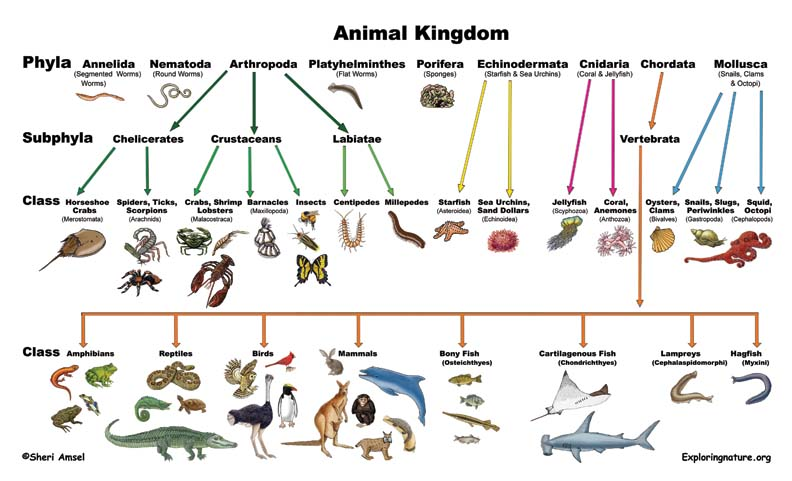
\includegraphics[width=0.85\textwidth]{figures/animal_classification}
  \caption{Classification of animals. The image is extracted from Exploring Nature.}
  \label{fig:animal_classification}
\end{figure}

\FloatBarrier

The input data for a classification task is composed by a collection of records, the dataset. In the same time, each record, also known as an instance, is composed by a set attributes. From all these attributes there is one considered special, which is called the target attribute or the class label. Regular attributes can be both discrete or continuous values. For the values signed for the class label, however, they must be discrete. This characteristic is what distinguishes classification form regression. Table \ref{tab:clasiffication_table} shows a sample dataset for animal classification into the following categories: amphibian, bird, fish or mammal.

\begin{table}[!htp]
\centering
\begin{tabular}{ |c|c|c|c|c|c|c|c| }
\hline
Common Name & Hair & Feathers & Eggs & Milk & Aquatic & Legs & Class Label \\ \hline
antelope & Yes & No & No & No & No & 4 & mammal \\ \hline
catfish & No & No & Yes & No & Yes & 0 & fish \\ \hline
dolphin & No & No & No & Yes & Yes & 0 & mammal \\ \hline
dove & No & Yes & Yes & No & No & 2 & bird \\ \hline
duck & No & Yes & Yes & No & Yes & 2 & bird \\ \hline
elephant & Yes & Yes & No & Yes & No & 4 & mammal \\ \hline
flamingo & Yes & Yes & Yes & No & No & 2 & bird \\ \hline
frog & No & No & Yes & No & Yes & 4 & amphibian \\ \hline
fruit bat & Yes & No & No & Yes & No & 2 & mammal \\ \hline
gull & No & Yes & Yes & No & Yes & 2 & bird \\ \hline
herring & No & No & Yes & No & Yes & 0 & fish \\ \hline
kiwi & No & No & Yes & No & No & 2 & bird \\ \hline
lark & No & Yes & Yes & No & No & 2 & bird \\ \hline
lynx & Yes & No & No & Yes & No & 4 & mammal \\ \hline
mole & Yes & No & No & Yes & No & 4 & mammal \\ \hline
mongoose & Yes & No & No & Yes & No & 4 & mammal \\ \hline
newt & No & No & Yes & No & Yes & 4 & amphibian \\
\hline
\end{tabular}
\caption{Animal kingdom dataset.}
\label{tab:clasiffication_table}
\end{table}

Tan Pang-Ning et al. propose a more mathematical definition of classification stating that it is the process of learning a target function $f$, also known as classification model, that maps each attribute set $x$ to one of the predefined class labels $y$.

\begin{figure}[!htp]
  \center
  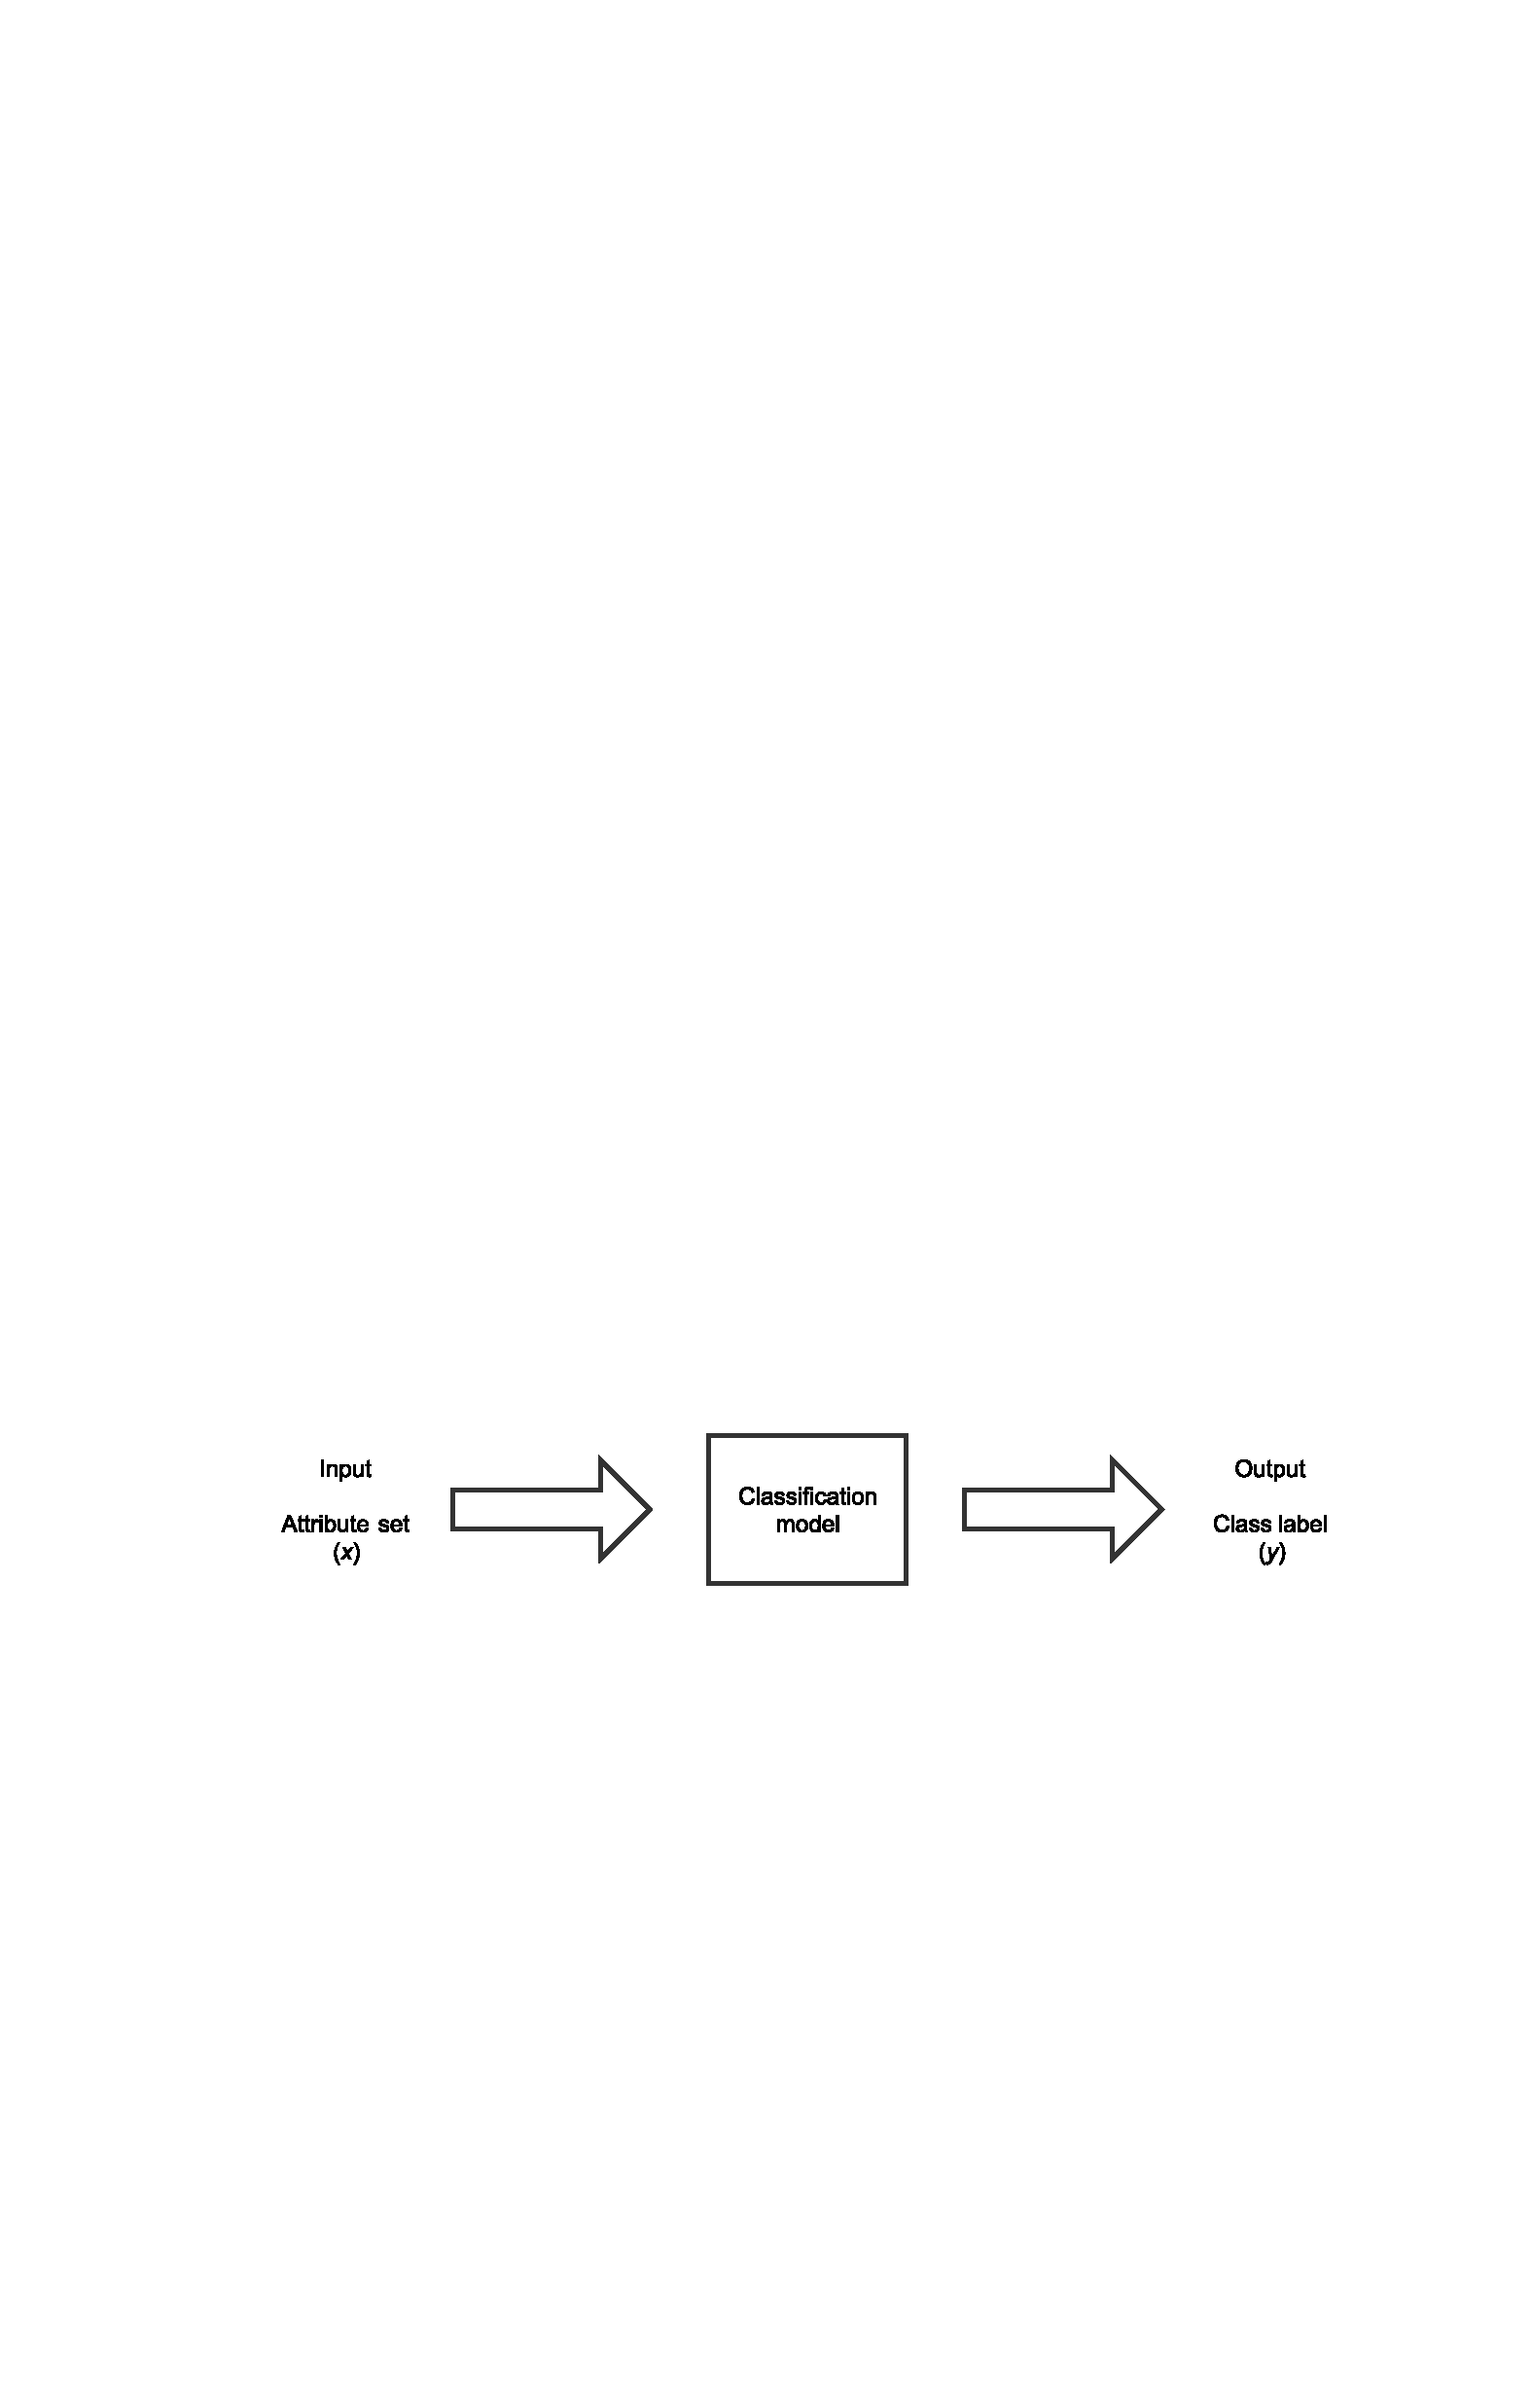
\includegraphics[width=\textwidth]{figures/classification}
  \caption{Classification as a task of mapping a set attributes $x$ into its fitting class label $y$.}
  \label{fig:classification_task}
\end{figure}

A classification model is useful for the following purposes \cite{pang2006introduction}:

\begin{itemize}
\item \textbf{Descriptive Modeling:} Since a classification model presents the main features of the data, it can serve as an explanatory tool to distinguish between instances of different categories \cite{madigan2002descriptive}.

\item \textbf{Predictive Modeling:} A classification model can also be used to predict the class label of an unknown new instance. As shown in Figure \ref{fig:classification_task}, a classification model can be represented as a black box that automatically assigns a class label to an instance by providing its attribute set.
\end{itemize}

It is important to remark that classification techniques perform their best when used for predicting or describing datasets which its class label is binary or nominal, Since they no consider properties such ordinality or the implicit order among the categories, they become ineffective with ordinal class labels \cite{frank2001simple}.

\subsection{General classification problem solving}
\label{general_classificartion_problem_solving}

For general classification problems solving, popular techniques consists on a process that starts with building classification models from a sample dataset \cite{witten2005data}. Each technique depends on a learning algorithm witch is in charge of generating the classification model. A good model should define the relationship between the input attribute set and its belonging category that suits the best. Therefore the model should be valid for both, the sample data used to generate the model and also for new unknown instances. Among popular classification techniques \acrfull{svm}, \acrfullpl{nn}, Naive Bayes or \acrfullpl{dt} can be found \cite{garje2016sentiment}.

\begin{figure}[!htp]
  \center
  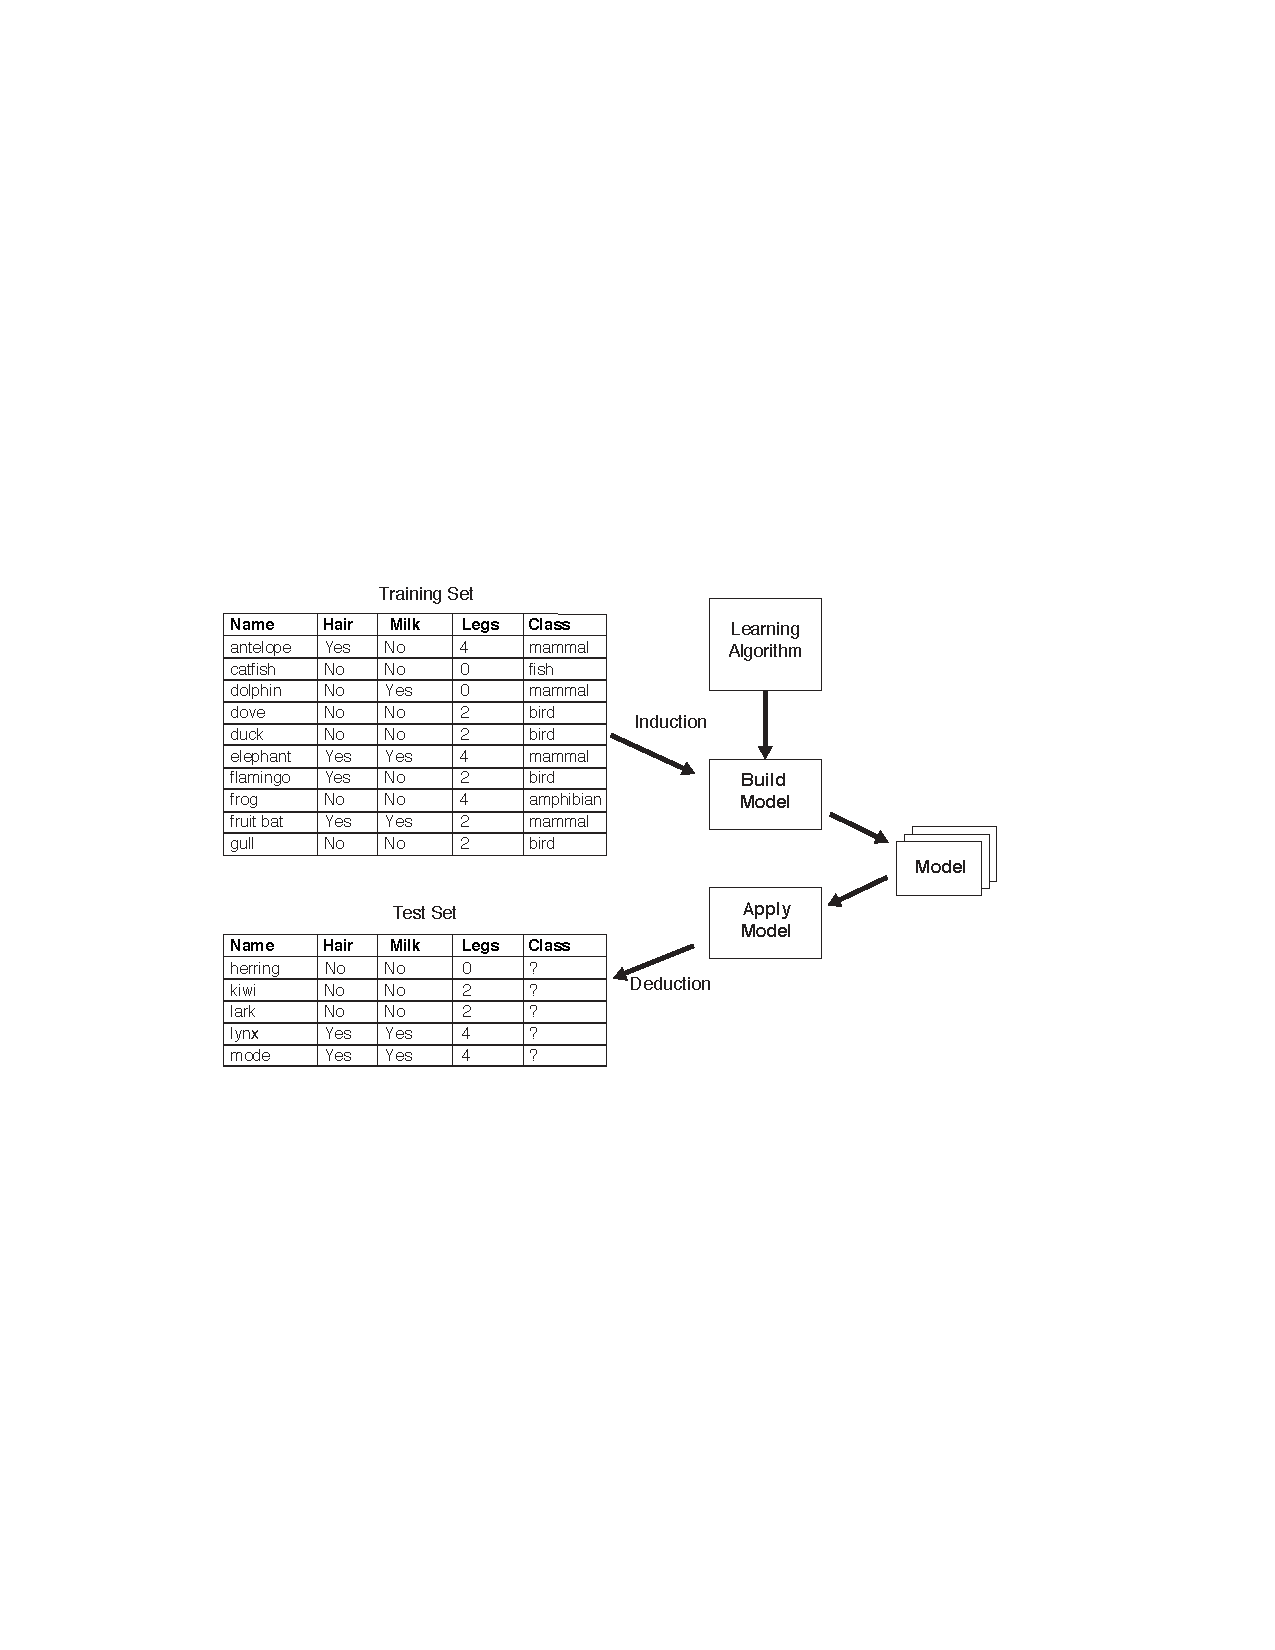
\includegraphics[width=0.85\textwidth]{figures/classification_problem_solving}
  \caption{General approach for classification model building and new instance category prediction.}
  \label{fig:classification_problem}
\end{figure}

As shown in the Figure \ref{fig:classification_problem}, to solve a classification problem a sample dataset must be provided as a training set. This sample is used to build the classification model according to the learning algorithm. After the model is built, it is applied to unlabeled dataset, also called the test set, to predict the categories of each instances of the records. To measure how good the model is, there is only need to count the number of instances have been correctly and incorrectly classified from the test set. Usually, to represent system's performance values, a confusion matrix is used \cite{hamilton2000confusion}. 


\begin{table}[!htp]
\centering
\begin{tabular}{ |c|c|c|c| }
\hline
\multicolumn{2}{|c|}{} & \multicolumn{2}{c|}{Predicted Class} \\
\hhline{~~--}
\multicolumn{2}{|c|}{} & $Class = Yes$ & $Class = No$ \\ \hline
\multirow{2}{*}{Actual Class} & $Class = Yes$ & a & b \\
\hhline{~---}
& $Class = No$ & c & d \\
\hline
\end{tabular}
\caption{Confusion matrix of a binary classification.}
\label{tab:confusion_matrix}
\end{table}

As a example, Table \ref{tab:confusion_matrix} represents the confusion matrix of a binary classification problem, in which the possible classes that can be assigned to a given instance are \textit{Yes} or \textit{No}. The values presented in this confusion matrix represents the counts of instances correctly and incorrectly classified as a means of model performance evaluation, being the diagonal of the table the instances classified correctly, the true positives (\acrshort{tp}) and negatives (\acrshort{tn}). The rest of the table corresponds to the number of instances that have been classified incorrectly, the false positives (\acrshort{fp}) and false negatives (\acrshort{fn}). The definition of a cell done by the value of the column and the row in which is positioned, read as the number instances of \textit{X} classified as \textit{Y}, where \textit{X} and \textit{Y} are the determined value of the row and column respectively. For instance, the cell $a$ is interpreted as the counts of Yes that have been classified as \textit{Yes}, the TP.

Although the confusion matrix gives all the relevant information to determine how well the system has performed, sometimes is convenient to provide this information into a single value that summarizes the content of all the table. To do so, multiple performance metrics have been defined and one of those is the accuracy defined as:

\[Overall\ accuracy=\frac{TP+TN}{TP+FP+FN+TN}\]

Accuracy represents the percentage of correctly classified instances. However, using only accuracy may not be enough, as for example when the dataset is imbalanced or it has a majority of elements for a determined class. Of instance, on a naive classifier that always determined an instance as the element with the maximum number of appearances in the dataset, the accuracy of classifier results in a high value although, the model does not have predictive capacity. This is considered the accuracy paradox \cite{accuracyParadox} and thus, to avoid the scoring a misleading measurement, it is recommendable to combine its usage with other performance metrics such as precision and recall.

Translating the precision from information retrieval context it would answer to the question \textit{how many classified items are relevant for the current query?} and thus, the precision is defined as:

\[Precision=\frac{TP}{TP+FP}\]

In the same context recall, in the other hand, answers to the question \textit{how many relevant items are classified properly?} and such, defined as:

\[Recall=\frac{TP}{TP+FN}\]

Finally, a combination of both measures, precision and recall, as a weighted average is called F-Measure or F1-Score. It allows to have a single performance metric to evaluate the classifier. Although, multiple definitions of the metric that give more relevance to the recall over the precision or vice versa exist, the general definition can be specified by the following equation:

\[F_1=2 \times \frac{precision \times recall}{precision+recall}\]

\iffalse

\subsection{Support Vector Machine}

There are four main advantages: Firstly it has a regularisation parameter, which makes the user think about avoiding over-fitting. Secondly it uses the kernel trick, so you can build in expert knowledge about the problem via engineering the kernel. Thirdly an SVM is defined by a convex optimisation problem (no local minima) for which there are efficient methods (e.g. SMO). Lastly, it is an approximation to a bound on the test error rate, and there is a substantial body of theory behind it which suggests it should be a good idea.
The disadvantages are that the theory only really covers the determination of the parameters for a given value of the regularisation and kernel parameters and choice of kernel. In a way the SVM moves the problem of over-fitting from optimising the parameters to model selection. Sadly kernel models can be quite sensitive to over-fitting the model selection criterion \cite{cawley2010over}

--------------------

SVMs are a new promising non-linear, non-parametric classification tech- nique, which already showed good results in the medical diagnostics, optical character recognition, elec- tric load forecasting and other fields.

Suitable for binary classification tasks.

The advantages of the SVM technique can be summarised as follows \cite{auria2008support}:

\begin{enumerate}
\item By introducing the kernel, SVMs gain flexibility in the choice of the form of the threshold separating solvent from insolvent companies, which needs not be linear and even needs not have the same func- tional form for all data, since its function is non-parametric and operates locally. As a consequence they can work with financial ratios, which show a non-monotone relation to the score and to the probability of default, or which are non-linearly dependent, and this without needing any specific work on each non-monotone variable.
\item Since the kernel implicitly contains a non-linear transformation, no assumptions about the functional form of the transformation, which makes data linearly separable, is necessary. The transformation oc- curs implicitly on a robust theoretical basis and human expertise judgement beforehand is not needed.
\item SVMs provide a good out-of-sample generalization, if the parameters C and r (in the case of a Gaussian kernel) are appropriately chosen. This means that, by choosing an appropriate generalization grade, SVMs can be robust, even when the training sample has some bias
\item SVMs deliver a unique solution, since the optimality problem is convex. This is an advantage compared to Neural Networks, which have multiple solutions associated with local minima and for this reason may not be robust over different samples.
\item With the choice of an appropriate kernel, such as the Gaussian kernel, one can put more stress on the similarity between companies, because the more similar the financial structure of two companies is, the higher is the value of the kernel. Thus when classifying a new company, the values of its financial ratios are compared with the ones of the support vectors of the training sample which are more similar to this new company. This company is then classified according to with which group it has the greatest similarity.
\end{enumerate}

--------------------------

Furthermore, $K(\bm{x}i, \bm{x}j ) \equiv \phi(\bm{x}_i)^T \phi(\bm{x}_j)$ is called the kernel function.

four basic kernels \cite{hsu2003practical}:

\begin{itemize}
\item \textbf{Linear:} $K(\bm{x}_i,\bm{x}_j) = \bm{x}^T_i \bm{x}_j$.
\item \textbf{Polynomial:} $K(\bm{x}_i,\bm{x}_j) = (\gamma \bm{x}^T_i \bm{x}_j + r)^d, \gamma > 0$.
\item \textbf{Radial Basis Function (RBF):} $K(\bm{x}_i,\bm{x}_j) = \exp(−\gamma \lVert \bm{x}_i − \bm{x}_j \rVert ^2),\gamma > 0$.
\item \textbf{Sigmoid:} $K(\bm{x}_i,\bm{x}_j) = \tanh(\gamma \bm{x}^T_i\bm{x}_j + r)$.
\end{itemize}

Here, $\gamma$, $r$, and $d$ are kernel parameters.

--------------------------

Support vector machines (SVM) were originally designed for binary classification \cite{hsu2002comparison}.

solving multi-class SVM in one step: “all-together” methods: [25], [27] and [7]. We then compare their performance with three methods based on binary classifications: “one-against-all,” “one-against-one,” and DAGSVM [23]. Our experiments indicate that the “one-against-one” and DAG methods are more suitable for practical use than the other methods. 

--------------------------

asdasdasd \cite{berwick2003idiot}

\begin{figure}[!htp]
  \center
  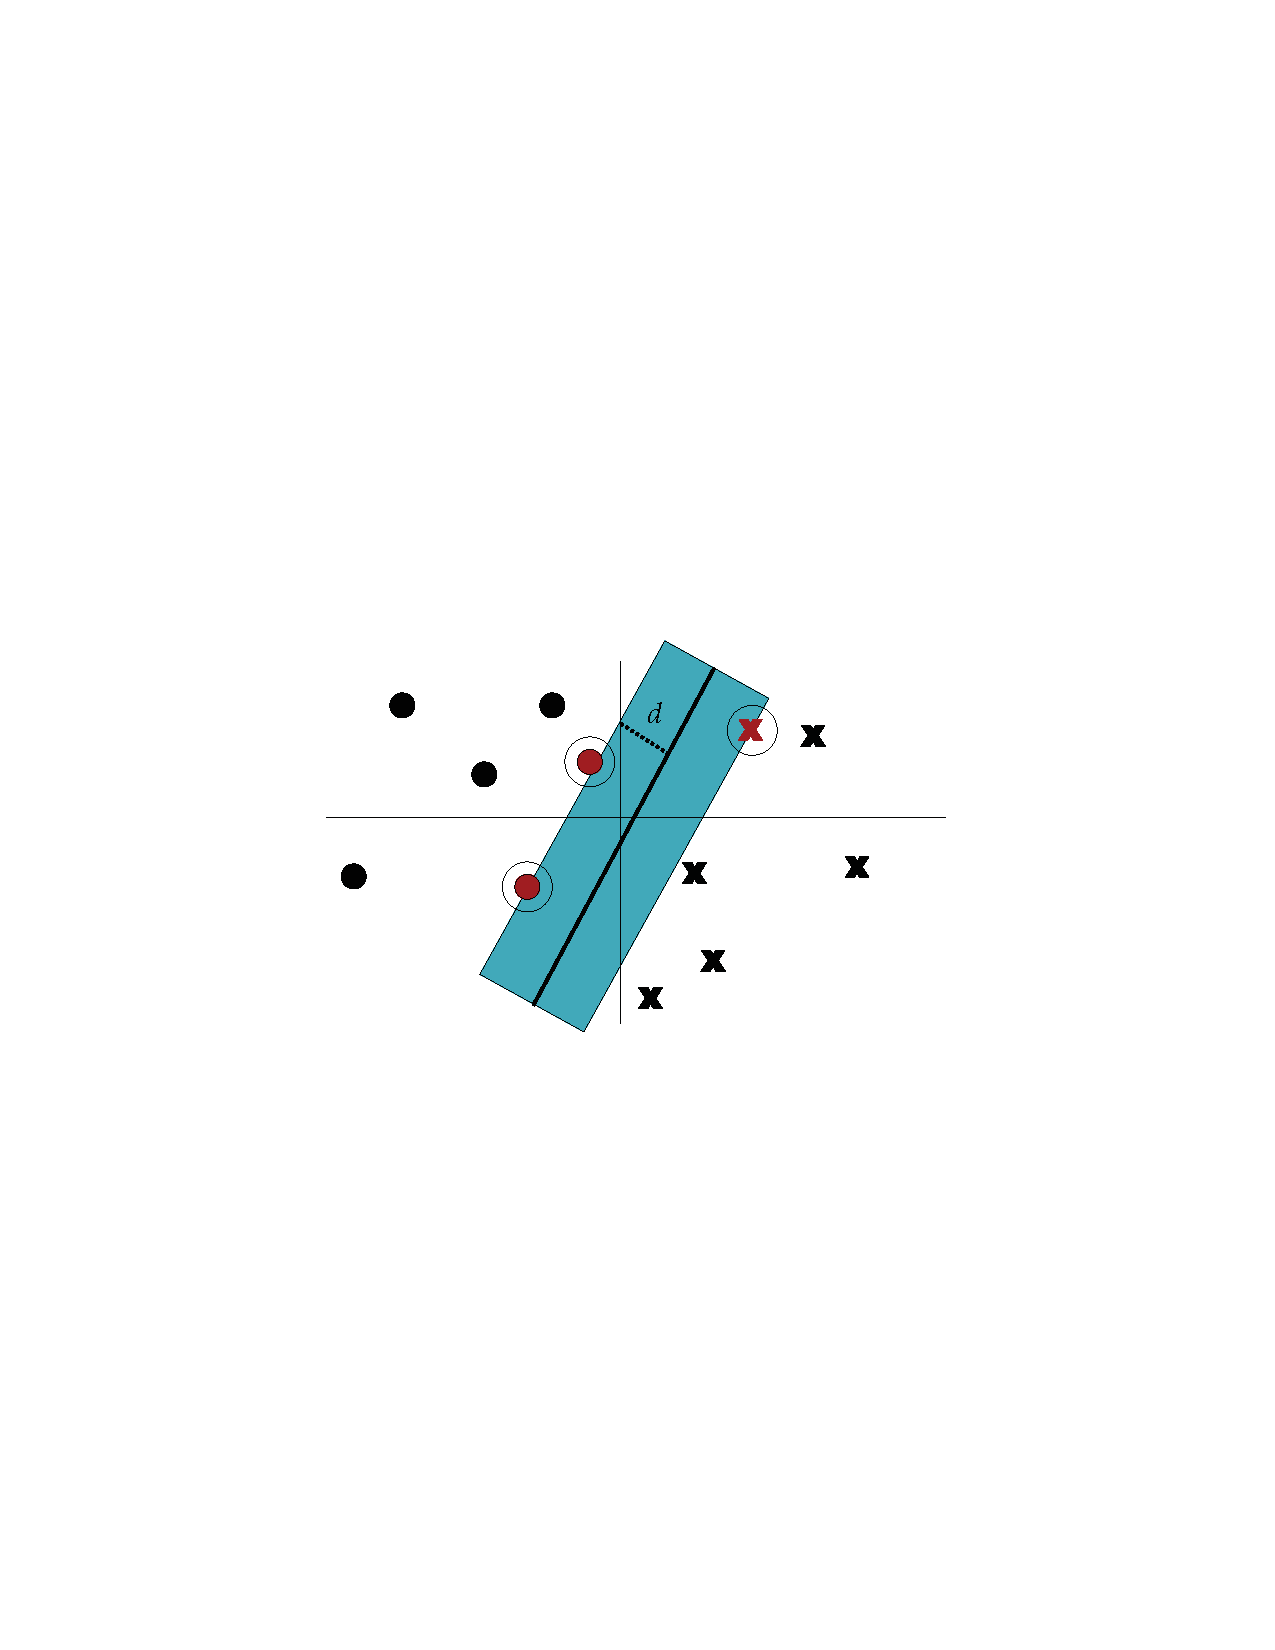
\includegraphics[width=0.6\textwidth]{figures/hyperplane}
  \caption{hyperplane}
  \label{fig:hyperplane}
\end{figure}

\subsection{K-Nearest Neighbor}

\subsection{Neural Networks}

\subsection{Ensemble Learning}
\label{subsec:ensemble_learning]}

\cite{ensemble2009Polikar}

\fi

\subsection{Deep Learning: Convolutional Neural Network}
\label{subsec:deep_learning}

In this section we will explain the fundamental of the algorithm on which the our solution is basen on, \acrlong{cnn}, a technology that was designed thinking mainly on computer vision tasks, but has proven to also for well on \acrshort{nlp} \cite{zhang2015sensitivity}, \cite{kim2014convolutional}. To understand how \acrshort{cnn} work, first we need to understand what a convolution is.

\section{Convolution}

A convolution could be defined as an integral that denotes the amount of overlap that the function $g$ shifts over another function $f$ (see figure \ref{fig:representation_convolution}).

Mathematically, a convolution is the product of two functions $f$ and $g$, depending on the values of the overlap are finite or not, the convolution (single dimension) could be defined as \cite{convolution}: 

\begin{figure}[!htp]
  \center
  \[[f \ast g](t)=\int_{0}^{t} f(\tau)g(t-\tau)d\tau\]
  \caption{Convolution for a finite range of $t \in [0, \infty]$}
  \label{fig:convolution_finite_range}
\end{figure}

or as:

\begin{figure}[!htp]
  \center
  \[f \ast g \equiv \int_{-\infty}^{\infty} f(\tau)g(t-\tau)d\tau\]\[=\int_{-\infty}^{\infty} g(\tau)f(t-\tau)d\tau\]
  \caption{Convolution for a infinite range of $t \in (-\infty, \infty)$}
  \label{fig:convolution_infinite_range}
\end{figure}

\begin{figure}[!htp]
  \center
  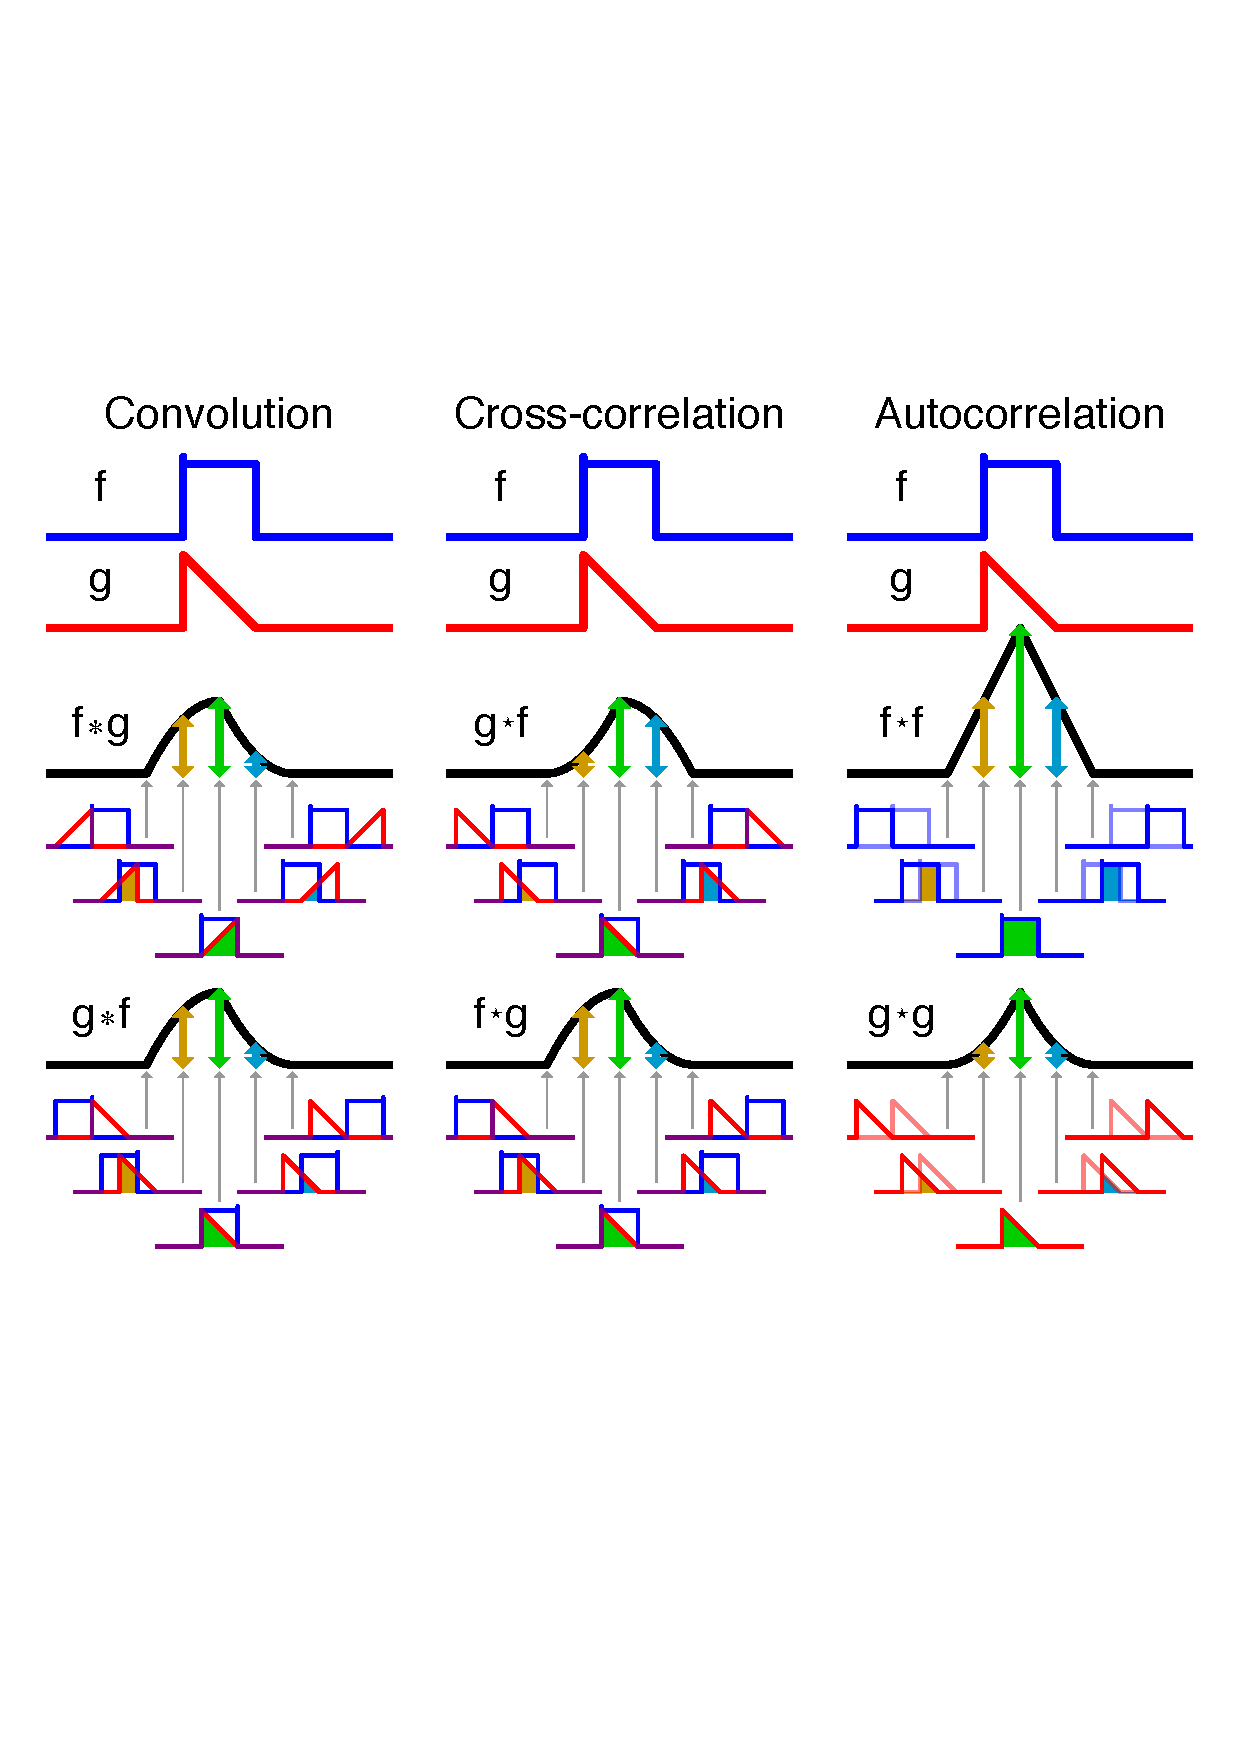
\includegraphics[width=0.6\textwidth]{figures/comparison_convolution_correlation}
  \caption{Graphical representation of a convolution and its comparison with correlation, image extracted from Wikipedia commons.}
  \label{fig:representation_convolution}
\end{figure}

A multidimensional convolution of infinite range the definition becomes \cite{multidimensionalConvolution}: 

\begin{figure}[!htp]
  \center
  \[f(t_1,t_2) \ast g(t_1,t_2) = \int_{t_1=-\infty}^{\infty}\int_{t_2=-\infty}^{\infty} f(\tau _1,\tau _2)g(t_1-\tau _1,t_2-\tau _2)d\tau _1 d\tau _2\]
  \caption{Multidimensional convolution for infinite ranges of $t_1,t_2 \in (-\infty, \infty)$}
  \label{fig:multidimension_convolution_infinite_range}
\end{figure}

In computer vision, images are transformed into two-dimensional functions, that can be represented as a matrix in which each value usually takes 0 or 1 values for black and white images or from 0 to 255 to gray-scale images. Most of the image transformation are based sliding window or function called ``kernel'', ``filter'' or ``feature detector'' \cite{cnnDennyBritz}, represented in figure \ref{fig:convolution_filter}.

\begin{figure}[!htp]
  \center
  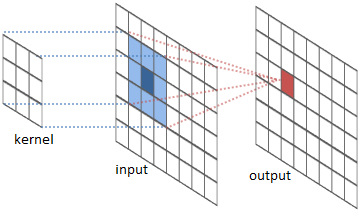
\includegraphics[width=0.6\textwidth]{figures/convolution_filter}
  \caption{Representation of a 2D image convolution transformation of filter size 3x3.}
  \label{fig:convolution_filter}
\end{figure}

\section{Convolutional Neural Networks}

\acrlong{cnn} are usually feed-forward type neural networks that concatenate multiple layers of convolutions with non linear activation functions as shown in figure \ref{fig:cnn_architecture}. The learning process of, for example, an image classification, learns the values by detecting the edges of the raw pixel values in the input of the \acrshort{cnn}. Over the following layers with the extraction of high level features, until reaching to last layer in which, all the fully connected layer classifies the objects by using the previously extracted features. 

\begin{figure}[!htp]
  \center
  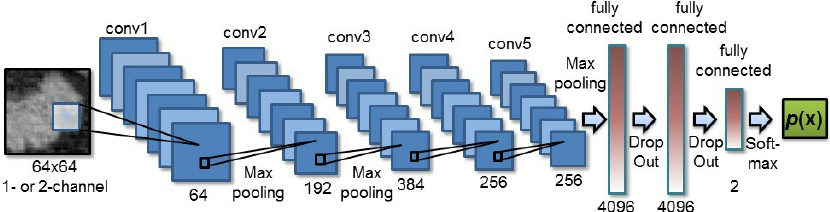
\includegraphics[width=0.96\textwidth]{figures/cnn_architecture}
  \caption{Example of a Convolutional Neural Network architecture \cite{kooi2017classifying}.}
  \label{fig:cnn_architecture}
\end{figure}

To apply the following architecture to \acrshort{nlp} related tasks, instead of a two convolution array that represents the image, each row of the matrix represents a token, usually being this tokens numerical representations of words or characters initialized with space vectors that are initialized with word2vec or GloVe algorithms. Then as with images each convolution layer extract features that are used on the last layer to categorize the given document as shown in figure \ref{fig:cnn_npl}. 

There are multiple types of architectures that combine multiple pooling layers that reduce computation cost by sub-sampling the matrix on each filter. In addition, as done in image processing, multiple channels of \acrshort{cnn} could be used to process each color, this idea can also translate into \acrshort{nlp} tasks by processing different word embeddings in each layer or applying different filters per channel \cite{singhalborrow}.

\begin{figure}[htbp]
  \center
  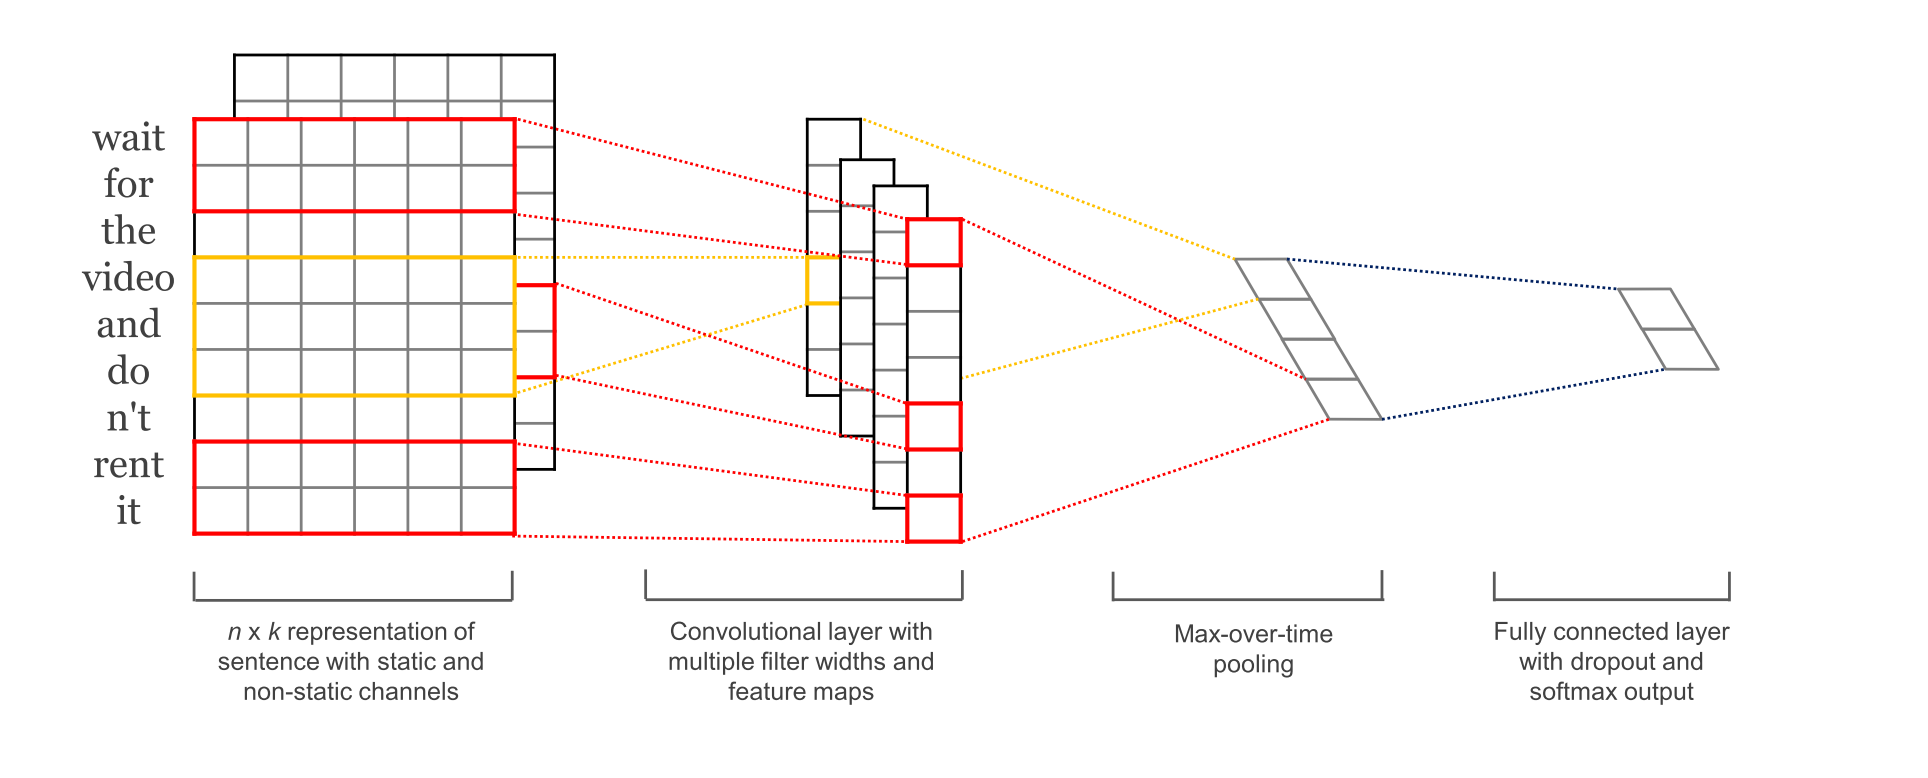
\includegraphics[width=0.7\textwidth]{figures/cnn_npl}
  \caption{Example of a Convolutional Neural Network architecture applied to NLP \cite{kim2014convolutional}.}
  \label{fig:cnn_npl}
\end{figure}

\chapter{Development}

SMILE Twitter emotion dataset\cite{wang2016smile}

"If you provide Content to third parties, including downloadable datasets of Content or an API that returns Content, you will only distribute or allow download of Tweet IDs and/or User IDs."\cite{twitterTOS}

EMOTEX\cite{hasan2014emotex} 

Twitter sentiment datasets are publicly available in CrowdFlower's ``Data for Everyone'' collection\cite{CrowdFlowerDfE}.

Wang dataset\cite{wang2012harnessing}

As stated on last sub-meeting, SemEval Workgroup's\cite{SemEvalPortal} labeled dataset doesn't work for the scope of this research. They focus on classifying polarity of texts messages (positive, negative and neutral classes) 
Time spending activity: Search for emotion related dataset.
 Found SMILE dataset, containing 3085 Twitter messages.
Classifies tweets into the following 7 classes: Anger, Disgust, Happy, Sad, Surprise, No-code and Not-relevant.

SMILE Dataset problems

Very small dataset.
More that 50\% of Neutral/"Garbage" data.
Multilingual tweets found (English, French, Japanese, among others.)
Almost 2\% of the data refers to Anger

Conclusions:
Not appropriate or enough for a decent supervised learning approach.

However English Angry tweets will be extracted for further use.

[Dataset class distribution image]

Research: Building automatic labeled corpus

EMOTEX \& SocialCom: search for tweets with Emotion hashtags from Circumplex model and WordNet Synsets.

[image of EMOTEX system to automatically obtain labeled]

Common Anger Hashtags:
\#angry, \#annoyed, \#annoying, \#bothered, \#frustrate, \#fury, \#furious, \#irritating, \#mad, among many others.

Twitter has made very specific restrictions on redistributing Twitter data, which means that available datasets don't include Tweet text, just a unique identification number.

Retrieve tweet text: python Tweepy\cite{Tweepy} API's .get\_status(id) method should do the work.

CrowdFlower public emotion dataset found!

[Data for everyone image]

Crowdflower emotion dataset statistics

40,000 rows of data.
Each row represents a tweet.
13 labels (classes)
Classification: 110 as Anger and 1311 as Hate. Sum: 1421 (3\%)

Conclusions:
Might be a good sample to do a binary classification test:

E.g. 1421 Anger / 1421 Not Anger (others)

Understanding WEKA ARFF file format

Up to now, downloaded datasets were stored as JSON, CSV or Plain Text files. However, WEKA works with a proprietary format file called Attribute-Relation File Format (ARFF).

Completed Task:
Convert downloaded CSV and JSON datasets to ARFF and load them into WEKA to check for possible conversion errors.

(python liac-arff module)

[ARFF file format explanation]

Some simple tests done

Testing WEKA's StringToWordVector to convert ARFF file's tweet messages into more machine learning friendly numerical attributes. (Combined with rainbow stopwords, stemmers, n-gram tokenizers)
Reading about how Random Forest algorithm works and use it to make a rough training and cross-validation classification with random selected features. (5 fold cross-validation results 28.49%)
Resample (Splitting original dataset into, training, validation and testing sets)
Weka's Attribute selection to predict best feature subset (wrappers and rankings) without overfitting.

Next week work

As Crowdflower dataset is composed of 40,000 instances, the resulting matrix from executing WEKA's StringToWordVector tool generates over sparse 10,000 features/attributes without filtering.
Classification of a such a big dataset using SVM or such algorithms takes over 2 hours in generating just the model (on a macbook pro laptop).
Therefore previously proposed 2,841 instances (1421 Anger / 1421 Not Anger) dataset is going to be built in order to be able to test those algorithms in reasonable time.

At the same time while testing new algorithms, information about how they work is going to be read, to understand if the obtained result are the expected.

Continue investigating WEKA and the useful tools it provides for text classification.

Crowdflower emotion dataset is unbalanced

Binary Classification Dataset Generation

Review  Anger and Hate classes and analyse the viability of merging them into a single class.
Checked both classes’ messages, they contain similar information. Therefore the merge is feasible.
Transform the leftover classes into “no anger” class to perform binary classification.
To solve the unbalanced dataset problem there 2 possibilities were studied: 
Use Stratified K-Folds. 
Undersampling the dataset to a more suitable class appearance ratio. (Random permutation of [No. angry tweets] without replacement)
Merge both classes randomly.
Text preprocessing (remove URLs, user mentions, etc.)

Last review’s result:
40,000 instances.
Word2vector, 1-3 n-grams\cite{cavnar1994n} (\~7000 attrs.)
Multi-class classification.
Random Forest (5 CV): 28.49%
This review’s results:
2,866 instances.
Word2vector 1-3 n-grams (\~5000 attrs.)
Binary classification.
Random Forest (10 CV): 63.89%
SVM\\SMO (10 CV): 65.42%
K-NN\\IBK (10 CV): 55.76%
NN (10 CV): Too long (cancelled)

[binary anger dataset distribution image]

Read literature about Convolutional Neural Networks for NLT\cite{cnnDennyBritz}

Use case of CNN for Computer Vision and its translation into NLP.
What is Convolution.
What are Convolutional Neural Networks.
Application into NLP.
CNN Hyperparameters:
Narrow/wide convolution.
Stride size.
Pooling layers.
Channels.

IMPORTANT: The input layer of CNN is a sentence composed of concatenated word2vec word embeddings.

Word2Vec on ksl-xe5: Preparing for DL

[Remainder] Up to know all the experiments have been done with WEKA’s GUI client and its automatic WordToVector tool.
Now a test using gensim (python word2vec module) has been done for the crowdflower multilabel dataset.
For the trained Word2Vec model, the GoogleNews-Vector(300)\cite{googleWord2Vec} has been used.

publicly available in: \href{https://drive.google.com/file/d/0B7XkCwpI5KDYNlNUTTlSS21pQmM/edit?usp=sharing}{GoogleNews-vectors-negative300.bin.gz}.
Output: 40,000 instances of arrays 31 elements (length of largest sentence for dataset) of 300 features. \~1.27Gb (Untabbed)
Spent time on research how to optimize serialization.
JSON default module Avg. time: \~ 16 mins.
UJSON module Avg. time: < 2 mins.

Expanding the dataset

Found another dataset (Wenbo Wang) that contains labels and tweet id.
Created a Twitter Application to have access to Twitter’s API.
Created a Python module that download tweets based on an id and save all the relevant data into a CSV. (Haven’t tested serialization yet, still downloading.)
This module can be expanded to become a streamer that download tweets based on emotion related hashtags, and get automatic labeled dataset as EMOTEX and SocialCom suggests.

Future Work: Create a CNN

Make a first test for a Deep Learning technique on the ksl-xe5 server.
Since the server does not have graphic cards to speed up the process, I will try to establish connection with my Home server in Spain and replicate the same environment and analyze if there is any performance improvement compared to CPU only computation.
Continue rating the chapter about how traditional classification algorithms work.

Some authors define sarcasm as a sub-set of irony.

Specs:
CPU: Intel I7-5930K (6 core/ 12 threads)
GPU: x2 GTX 980TI (5.63 TFLOPS)
Storage: 1TB Samsung 950 PCI-E SSD Raid 0

Tweet downloader: Wang Dataset

Successfully tested programed module to download Wang dataset. Download tweets into CSV with the following information:
tweet-id, label, author, text-content
However, since dataset is formed with tweets collected from 2011, some of the are unavailable. E.g. From the test.txt, which originally contains 250,000 tweets only 65,324 has been able to be downloaded. (Took 30 hours to download)

TODO: Implement a logger to check if the tweet could not be downloaded due to unavailability or a network failure, for a download retrial.

Started implementing the CNN

Started implementing the Convolution Neural Network (CNN) by using Keras\cite{keras} python module for Deep Learning.
Just need to make some adaptations to the way it parses the word2vec values to be able to test it.
I also investigate how to make full use of the dual graphic card setup of my home server. According to literature I have read there are two techniques to distribute the workflow:
Data parallelization
Model parallelization
The technologies used are based on Message Passing Interface (MPI) architecture. Apparently is not a simple task and the speed up rounds x1.3~x1.6 (last percentage being very unlikely)

Work for next week

Implement the tweet downloader logger to understand why downloads fail, and try to re-download them if network failure.
Finish implementing the CNN.
Do a single GPU test with home server and measure required time to perform the classification.

Tweet downloader

Implemented a basic logger that stores in real time the tweet\_id, error\_code and message on a file. With this simple logger I found these possible errors:
Error 34: Sorry, that page does not exist.
Error 63: User has been suspended.
Error 88: Rate limit exceeded.
Error 114: No status found with that ID.
Error 179: Sorry, you are not authorized to see this status.
Error 500: Internal Server Error.

Error handling (1)

For the previously presented error list there are only two errors that can be handled:
Error 88: Rate limit exceeded.
Error 500: Internal Server Error.
Twitter API enables to download tweets for an interval of 15 minutes, after that it stops providing data for a server request cold down. To solve this error, I make the tweet downloader to wait until the server sends a download acknowledge to resume the download process and avoid getting tweets lost during the cold down interval.

Error handling (2) and logger optimization

Since the Internal Server Error can happen randomly and its duration of the error is unpredictable, the error is recorded for posterior tweet redownload.
As real time loading involves serialization of small chunks of information multiple time, and the error code and message gets repeated it become inefficient and slow down the tweet download. The solution proposed consists on producing a dictionary in RAM and save it into a JSON file with the following structure after the download finishes:

$...
‘code-error (key)’: {
‘tweets’: [
	tweet\_id,
	tweet\_id
	...
]
‘message’: message text.
},
‘No-code-error-message’: {
	‘tweets’: [
	tweet\_id
]
}
...$

Measuring performance

First downloading test consist on downloading tweets from labeled tweet id list. Originally it contained 250,000 tweets. The system was able to download 65,324 tweet text in 30 hours.
After handling the server cold down error the system was able to download 153,387 tweets in 69 hours.
The system maintained almost the same performance after adding the having added the error logger comparing the time spent with the amount of tweets downloaded.

Deep Learning

First basic Deep Learning test implemented using Convolutional Neural Networks (CNN) on Crowdflower multilabel dataset (Keras over TensorFlow). From 40,000 tweets 70\% has been used for training and the remaining 30\% for validation. Has is the first test, 3-grams, 4-grams and 5-grams have been used for the training over the 300 attribute word2vec. Every convolution generates a set of features, but they are discarded for now.
This week I have been able to test on ksl-xe5 server. The results obtained on the training validation accuracy disappointing for 13 label classification, about 26.33\%. It spent 4 hours 30 mins for the training task for 40,000 tweets.

Model characteristics:
Model size: 300
Number of filters: 200
Batch size: 50
Number of epochs: 1000
Evaluation period: 12

Work for the next week

Run the CNN test on home server and try to run on spain university for speed up checking.
Spent some time investigating test preprocessing such as English contraction expansion and misspelled words correction.
Investigate how to improve accuracy in classical and deep learning technique by exploiting features.

Last notes

I have contacted the vice-dean of University of Deusto and ask about how much time I can spend in NUT for the research. Their answer is that I can stay as much time needed, following NUT’s evaluation schedule. 
Meaning that if NUT accept it I could extend my stay in Japan for research as much I NUT allows me.

Deep Learning CPU only vs GPGPU

Last week I was able to test the implemented Convolutional Neural Network on Crowdflower multilabel dataset, based on a TensorFlow and Keras modules.
Using a CPU only configuration on ksl-xe5 server it took 4 hours and 30 minutes to complete the training and validation over the 40,000 tweets.
On the home server running the same test on a GPGPU configuration in conjunction with CUDA 8 and CUDA Deep Neural Network (cuDNN) v5\cite{chetlur2014cudnn}, it took 2 hours 9 minutes to perform the same task. Proving that GPGPU can speed up 52.59\% the process.

Model characteristics:
Model size: 300
Number of filters: 200
Batch size: 50
Number of epochs: 1000
Evaluation period: 12

Test processing
Investigated about expanding unambiguous English contractions to process them into word embeddings. After using a dictionary of contractions and being able to expand them I found that NLTK Stopwords would remove them anyways. A future task would be to investigate if negation is a good feature to extract and if so, remove them from the Stopwords list to the able to process them.
I also investigated Oxford’s Common Misspellings and PyEnchant, a python module that uses OpenOffice dictionaries to correct spelling errors. I will implement a test to check if I can correct misspellings and compare corrected words appearance with the pre-trained Word2Vect model.

Feature extraction

This week I’ve been focused investigating about emotional words lexicon and emoticon lexicon. I have download available lexicons from NRC Emotion Lexicon (EmoLex) and used Wikipedia’s and EMOTEX’s list of emoticons to create an emoticon lexicon. I have used Regular Expressions (regex) to find emoticons on tweets, before the punctuation removal.
The next step would be storing them into the word embeddings to make use of them on CNN, and as a feature for classical classificators.

Future work

During the training phase on the CNN the weights are now static, therefore I will investigate how to make this weights variable.
CNN only work with word embeddings, and do not support the use of other features as with classical classifiers. Due to this I will implement a SVM classifier and use the emoticons, appearance of emotion words, and other features apart from word embeddings.

Spelling check (1)

Last week I talked about a python module called Pyenchant, which provides a function suggest(word) returning an ordered list with the possible corrected words. However it’s accuracy is not very high. Therefore I researched new approaches and found an basic idea proposed from Peter Norvig\cite{PeterNorvigSpell}, Director of Research at Google Inc. He explained that Google search engine uses probability theory to choose the most likely spelling correction for a word (argmax).
argmaxc ∈ candidates P(c) P(w|c)
C ∈ candidates: Candidates model.
P(c): Language model.
P(w|c): Error model.

Spelling check (2)

Candidate model is limited to words with up to 2 editions, correcting splits, deletes, transposes, replaces and insertion errors.
The language model estimates the probability of a words by counting the number of appearance. The tests runs on a dictionary that uses Project Gutenberg’s free eBooks, Wiktionary most frequents words\cite{WiktionaryFL} and \acrfull{bnc} \cite{bncFLAdamK} (Model side ~6Mb.)
The error models prioritizes the original word if it is known, the the list of words known with one modification, followed by the list of words known with two modifications and finally the original word if it is unknown.

Spell checker result using the Big.txt Language Model that Norving Provides.
51\% of 270 correct (35\% unknown) at 37 words per second
53\% of 400 correct (32\% unknown) at 35 words per second

Using the Language Model I generated.
75\% of 270 correct (5\% unknown) at 64 words per second 
69\% of 400 correct (7\% unknown) at 63 words per second

Making some tests

I tested spell correction with the crowdflower dataset. Checking the word that were not numerical. Whenever the spell checker modified a word I printed into the screen so I could do a manual comparison.
I found that the accuracy was better than the enchant module but it continue failing in some cases and all the slang that people uses on the internet was missing in the model, therefore those kind of words were being replaced by a totally unrelated words.
The next step I made was investigating about english slang used on twitter and improving the model accuracy.

Improving the model and twitter slangs (1)

Since the model does not contemplate slang terms found on tweets I have searched for a dictionary of slang with their meaning, so that it can be replaced from the original text during the preprocessing.
To improve the model first I searched for some n-gram database. Google has a huge that includes 5-grams (~22Gb), However the access to this resource costs 150 USD for non-members\cite{LDCGoogle5-gram}. Therefore, I downloaded all the English Ebooks from Project Gutenberg as for 2014 from Kiwix harvester\cite{kiwix} (~42Gb) publicly available from \url{http://download.kiwix.org/zim/gutenberg/gutenberg_en_all_10_2014.zim}. After solving encoding errors in some file names I start the eBook preprocessing.

Improving the model and twitter slangs (2)

Since all the eBooks are stored as HTML document, I removed all the HTML tags from the texts, to improve later on model generation performance, it took 1 hour 38 mins to remove all the HTML tags.
I programmed a python module that take the requested model size as argument and concatenates as many eBooks until reaching requested size.
The Spell checker now read the model generated from this book concatenation, but next step would be to generate a word counter and store this document as a model instead to improve even more spell checker performance.

Future work

Put all spelling related modules and slang dictionaries together and test on crowdflower dataset to check if performance improves.
Continue emoticon and emotion words feature extraction.
Continue implementing weight variable Convolutional Neural Network training.
Continue implementing SVM classifier.

Spell checking model redesigned

On the previous I stated that I programmed a python module that removes the HTML tags from Project Gutenberg's eBooks and concatenates it into a single document to. Last week I redesigned this module.
Now, the program search for word frequency files from eBooks and generates a single dictionary with the word occurrences from each document.
If the word frequency file does not exists for a certain eBook it process the document by checking if it contains HTML tags and if so remove them, overwriting the original file in the process.
Calculates the word frequency for that eBook and saves it into a file while at the same time updating the global dictionary that contains the words for all documents.
This way if the program has to run a second time it does not have to start all the process from the beginning.

Adding twitter scope words to spelling model

After downloading 36,173 English eBook from Project Gutenberg\cite{projectGutenberg}, and the most general used word from wiktionary and oxford corpus I decided to add more content that its form could fit better to the written style used on twitter messages. Therefore I decided to add to the model the following list of most used words:
TV programs words from Wiktionary.
Film series from Opensubtitles extracted by Hermit Dave\cite{openSubtitlesFL}.
Contemporary fiction from Wiktionary.

Merge Datasets

Programmed a python module that receives as input a list of dataset paths and a sentiment target label “mapper” file. 
With this information perform a dataset concatenation, and transforms labels as the mapper file states and filter tweets that contains non-english characters, typical from Spanish, Portuguese and French, found on Wang dataset.
It can also transform the dataset labels into “anger” and “no\_anger” classes, used for binary classification.

Generalize Python Modules

Since all the programmed modules inputs and outputs were hardcoded, I spent time on making them variable arguments introduced on console line.
This would ease me testing the programmed modules with different datasets, such as word2vec transformation and Convolutional Neural Network (CNN) classification.

Convolutional Neural Networks Binary Classification Test

My last test with CNN I used Crowdflower’s dataset, consisting in 40,000 tweets with 13 sentiment target labels. The dataset was divided in 70\% training 30\% validation. After training the validation accuracy the system scored was 26.33\%. Then I made a second test using the spelling checker on the word2vec process. If a word could be found in the model it would check it’s spelling and replaced with the suggested word correction. The accuracy the system scored after apply this simple modification was 27\%. For my last test I decided to change the dataset. I merged Crowdflower’s dataset and Wang’s test.csv and transform it into a binary class label dataset, representing 33,752 “anger” and 33,752 “no\_anger” tweets. Again, using the spellchecker on word2vec process I run the CNN classification and obtained a 99.73\% validation accuracy.

Convolutional Neural Networks Binary Classification Test

Since the result were so good I thought I did something wrong, and check that the merged dataset was formed correctly without repeated data. But apparently it is OK. Therefore, since I didn’t have 21,000 tweets for creating proper size test dataset and I did not have time to retrain the model again and re-split the dataset, I took my remaining small “train” dataset I had from Wang dataset, containing 282 tweets. I made a binary dataset with that and used as test data. By using the model weight I got from the training and validation process I test the new unclassified 282 binary labeled tweets. The system achieved a 100\% accuracy on the testing phase over that small dataset.

Future work

Add slang dictionaries and test crowdflower dataset to check if performance improves.
Continue emoticon and emotion words feature extraction.
Continue implementing SVM classifier.
Split the dataset into 70\% train 15\% validation 15\% test and re-run the CNN module and recheck the results over binary classification.
Calculate Precision, Recall and F1-score.

Last week I made the first CNN accuracy evaluation that achieved 99.73\%, but the test size was 282 tweets, compared to 21,200 tweets used in the evaluation, which was not enough.
Due to that, I made modifications into the module that transform the dataset into word embeddings to be able to split the dataset into 70\% training, 15\% validation and 15\% testing.
Right away, I made another CNN training, and validation and testing, and confirmed that the accuracy was really of 99.73\%

CNN: Speed up training phase

During last test I made I realise that most of the time of the training phase, the model was not learning anything new, after the maximum validation accuracy was reached. Therefore I spent time or investigating how to stop the training phase when no more gain was scored. I found the following relevant classes:
EarlyStopping: Stop training when a monitored quantity has stopped improving (‘val\_loss’)
ModelCheckpoint: Save the model after every epoch. (Save only best model)
Spent time comparison:
Before modifications: \~9 hours 30 mins.
After modifications: \~10 mins. (Stopped after 22 Epoch)

Confusion Matrix and Scikit evaluation

To evaluate that what I was doing was right I created a confusion matrix with the method Keras library provided, plus what I researched about how to make diagrams with matplotlib’s pyplot. The result was this:

[image of confusion matrix]

Scikit evaluation\cite{scikit-learn}

Since I cannot the data I got from Keras I used scikit to check if the predictions CNN make are correct. I for the confusion matrix I was also able to calculate the following evaluation metrics:
Accuracy: 0.9974323524
Recall (macro): 0.9974325863
Precision (macro): 0.997434915
F1-score (macro): 0.9974323499

Cuda installation on arrived server (1)

I tried to follow my own installation guide I made several weeks ago and try to install Fedora 24. However, the combination of Skylake and Pascal architecture has made the more difficult.
Skylake requires Linux kernel 4.5.5 to work.
Fedora 24’s open-source video drivers don’t work with Pascal architecture, so after grub menu in the OS installation process the screen becomes black.
Therefore I tried to Install Fedora 25, that run’s wayland by default instead of X server. Nevertheless, I found that Nvidia does not support the kernel source that packs Fedora 25 and makes difficult its installation.

Cuda installation on arrived server (2)

So I decided that I would keep to my original idea to install Fedora 24. To do so I read that first I had to disconnect the Nvidia GPU out of the PCI slot. After almost 1 hour trying to pull out the GPU out of the board (It was stuck on the PCI port) I was able to run the Fedora 24 live USB and install it.
This week, I will check if there is any problem with kernel version and Nvidia. But if I find any problem that makes difficult the cuda toolkit installation, my last attempt will be to install Ubuntu 16.04

Future work

Add slang dictionaries and test crowdflower dataset to check if performance improves.
Continue emoticon and emotion words feature extraction.
Continue implementing SVM classifier.
Fix CNN accuracy lost after serializing model.
Install all CUDA Server’s dependencies.
Search for an irony dataset to make test with CNN.

Download Irony and Sarcasm tweets
Previously I read some literature about Irony and Sarcasm. Some authors define sarcasm as part of Irony. Others state that is a figurative language completely different. For my research due to the reduced amount of data I have found so far, I will deal with these term as if they were equal.
With the tweet-downloader module I have been able to download tweet that contain the \#irony, \#ironic or \#sarcasm hashtags in tweets. Up to now the system has downloaded 18,398 tweets, which I still need to preprocess and filter.

Preprocess Irony Dataset
I used a Google Sheets extension called Twitter Archiver that remotely downloads tweets and saves it into a Google Sheets document.
As I said on last group meeting, I was downloading English Tweets that contained \#irony, \#ironic and \#sarcasm hashtags.
I have managed to download a total of 34.000 tweets (still downloading)
I need to remove useless columns from the CSV, rename columns names to be able to use with my python modules, remove duplicate tweets documents (Retweets) and remove these 3 hashtags from the text.
I created a python module that performed all the tasks from last point.

Perform Irony Dataset CNN Test

Dataset characteristics:
Instances: 56,264 tweets.
Balanced 50\% irony (28,132)
2 target labels, (binary)
Split: 70\% train. 30\% val.
Val. Acc: 91.88\% (w/u spell)
Val. Acc: 91.86\% (w. spell. chckr)

Recall (macro): 0.9188087708
Precision (macro): 0.9188862312
F1 (macro): 0.9188298366

Note: With the spell checker the CNN losses accuracy for this dataset. To implement a more complex spelling checker would be needed, + other techniques (stemming, lemmatization, synonyms).

Model characteristics:
Model size: 300
Number of filters: 200
Batch size: 50
Number of epochs: 1000
Evaluation period: 12

Found a bug in Anger Dataset

Anger dataset is generated by merging the Crowdflower dataset and Wang test dataset.
When I created the dataset I checked that Crowdflower tweets didn’t contain hashtags such as \#anger, \#rage, etc. However I forgot to check that on the Wang dataset, which  DO contain them. I modified the dataset merger module to find those hashtags and remove them from the tweet content. After doing it a performed again the CNN to recheck the results:

Dataset characteristics:
Instances: 67,504* tweets.
2 target labels
Acc: 99.64\~99.74\%

Dataset characteristics:
Instances: 70,108 tweets.
2 target labels
Acc: 95.92\% (w/o spell)
Acc: 96.15\% (w. spell chkr)

Note: Used less tweets on first test because I removed all the duplicated tweets. Now the merger maintains the first instance. (fixed)

Future work
Investigate how to combine both anger and irony classificators and do a final test with that classifier. (Ensemble Learning?)

Continue implementing SVM classifier.
Add slang dictionaries and test crowdflower dataset to check if performance improves.
Continue emoticon and emotion words feature extraction.
Fix CNN accuracy lost after serializing model.

CNN module
After training and validating the model, serializing it and loading the weights for posterior executions would produce a considerable accuracy lost on the classifier (\~51\%). This issue has been already fixed. The possibility of storing the models and make the weights reusable enables to program successive module that uses all the pre-trained classifiers to combine their results to detect repressed anger tweets.
Fixed a bug with the Confusion Matrix Drawer, not rendering the normalized version of the matrix properly.
Standardized the output to easily be able to use the results into the next module that combines all classifiers.

Read literature (Model combination)

Since I have two classifiers that can detect anger and irony independently, I have read some papers about the techniques used to combine the classifiers to be able to use the to detect repressed anger. First I thought about Ensembled Learning’s Divide and Conquer technique, with a voting combination rule. However after Asking to Yukawa sensei he proposed to build a 2x2 matrix to classify the output as following (right):

[Image of divide and conquer technique]

[image of 2x2 combination matrix]

I started programming the module that combines the classifiers. It already loads the classifiers. However I have to preprocess the dataset on a different way to proceed with the prediction and combination.

[image of the merge to word2vec process]

Note: Combined test dataset fragment is used in the final step’s prediction phase.

Question:
Can the binary anger and binary irony datasets’ no\_irony and no\_anger have tweets in common?

Finished dataset preparation

[image of the merge to word2vec process]

Implemented the dataset preparation system that I presented last week.
Around unique 220,000 gathered after merging all datasets.
Re-splitted dataset into anger and irony binary dataset with no common tweets with 67,746 and 56,264 tweets respectively. (removing key hashtags)
Resulting dataset were divided into 73\% train, 18\% validation and 9\% test.
Anger and irony’s tests dataset were merged generating a the final prediction file of 11,060 tweets.

Pre-training the classifiers and prediction

Resulting train and evaluation word embeddings are used for classification learning process, generating model structure and model weights files.
Test word embeddings are used to generate an approximate performance record sample.
With the model structure and weights and the merged test dataset, a CSV with the prediction result is generated.
A evaluation method for this last step is still missing.

[image from word2vec to final prediction process]

Searching for evaluation method

[image of excel with the classification labels, half of the prediction can be done]

To validate the prediction, Yukawa sensei suggested to perform a manual classification of the dataset

Dataset manual classification

As doing a single classification is not reliable, I created a program with google app script that automatically creates google forms based on the dataset data.

I will send to some friends to help me with this task, in order to improve the reliability of the manual classification.

[various images of google tech, code, forms and results]

Doubt: Using hashtags or remove them

Example 1:

I \#hate when I have to meet my neighbors in the morning. (in sentence natural usage)

Example 2:

I had to explain my parents once again how to use the refrigerator due to Alzheimer \#sad 
(out sentence usage for classification)

The second usage case alters the results of the classification. But since I cannot differentiate between all the tweets of the dataset, I think that I should remove all the dataset, (even if some of the sentences lose meaning) because the second case (majority) is faking the result of the learning process. 

Re-run the learning process (no hashtags)

After re-running the learning process of both classifiers and check their individual accuracy score it when down to 78\% and 84\% for anger and irony respectively

Dataset manual classification

Since I generate a new random dataset with no hashtags I had to start the manual classification again.

Manually classified 300 tweets by myself. 

Collaborators have classified 100 tweets (validation).

My goal is to have at least 1000 tweets classified and validated.

Processing the form results (I)

Background: In the forms I asked 2 questions: (I) to classify the sentence and (II) if the sentence was from the irony tweet downloader task I also ask them if the tweet was really ironic instead of talking about irony. This would help me to correct the misclassified tweets in the automatic process.
Difficulties found by the classifiers:  
Some of the tweets are answers to other messages, without that context is difficult to classify current tweet properly.
To check if a tweet is ironic, on some tweets they lack information about the topic to judge properly.
After finished my part of the manual classification, while the collaborators keep sending me more form responses, I started programming the module that processes the results and incorporates them into my CSV for later use in the validation of the system.

[image of generated excel from google form responses]

Results

From the 11,074 tweets dedicated for the prediction phase 1,000 were manually classified. From the obtained responses only those tweets that more than half of the submitters were chosen, the rest (176) were considered ambiguous.
In the end the amount of tweets available for the evaluation process were 824 with the following distribution:
Explicit anger: 193, Irony: 47, Repressed anger: 44 and Normal: 546

[CHECK WHY AMBIGOUOUS NUMBER IS 176 BUT 830 TWEETS ARE IN DATASET INSTEAD 824]

Accuracy: 0.5144578313
Recall(macro): 0.4695591165
Precision(macro): 0.3846361992
F1-Score(macro): 0.3871343406

Trying a new pre-trained word2vec model (I)

Up to know I have been using Google’s publicly available 300 feature, pre-trained word2vec model that has been trained from the english text extracted from Google News.
However, this news tend to be written in a style that differs from how tweet are. Usually tweets contain terms used in spoken English that do not appear in the news. This is the reason why a important amount of theses words are not presented in the Google’s model. Apart from trying to correct the word spelling and use a slang dictionary, using a model that have been trained with actual tweets would increase the chances of improving the amount of words used on the dataset presented in the model.
I found a new model, from Fréderic Goding\cite{godin2015multimedia} that has been trained with 400 millions of tweets and uses 400 features.

Not enough RAM Memory

I encounter a few problems to run the whole process with the new model in two steps: (I) generating binary anger dataset’s word embeddings and (II) compiling the CNN for the first time to train the anger classifier. In both processes the ram of the current GPGPU system is enough to complete these tasks. 
For the word2vec module, before I the GPGPU system was ordered I was working with xe5 server with 128GB of RAM. Therefore, I focus the implementation of the module in execution speed, not on memory consumption. But for the GPGPU system, since the memory is limited I optimize it as much as I could without sacrificing the initial speed design. I managed to make it work with Google word2vec pre-trained module, but for twitter it is not enough.

Memory consumption and xe5 execution time
I run the word2vec over the binary anger dataset on xe5 and check its memory consumption check the amount of memory need to complete that task. The maximum peak was around 43GB of RAM. Since in this process only CPU and RAM are involved the execution time is more or less the same as in the GPGPU system.
For the CNN compilation and training the peak was 30GB of RAM on xe5. Even if the GPGPU does have 31.3GB of memory available, it does still crash. Forums on the internet refer to this error to not having enough RAM or powerful CPU. xe5 expent almost 2 hours to finish the training of the CNN. When the same task with binary irony dataset, that luckily does work under the amount of RAM (\~8,000 tweet less) available usually takes around 6 minutes.

Results comparison
Accuracy: 0.5626506024
Recall(macro): 0.4403748582
Precision(macro): 0.3916296856
F1-Score(macro): 0.390081225

[images of normalized confusion matrix from google and twitter model]
\chapter{Research Framework}
\chapter{Results}
\chapter{Conclusion and Future Work}
\chapter{Self-assessment}

\begingroup
\raggedright
\sloppy
\printbibliography[heading=bibintoc]
\endgroup

\printglossary[type=\acronymtype]

\appendix

%\input{contents/extra/Acknowledgements}

\backmatter

\end{document}


\makeglossaries

\appendix

%\input{contents/extra/Acknowledgements}

\backmatter

\end{document}